\lhead{Appendix B \emph{Magical Vectors and where to find them}}
\label{appendix:B}
This appendix contains extra figures from \autoref{Chapter5}
\begin{figure}
\centering
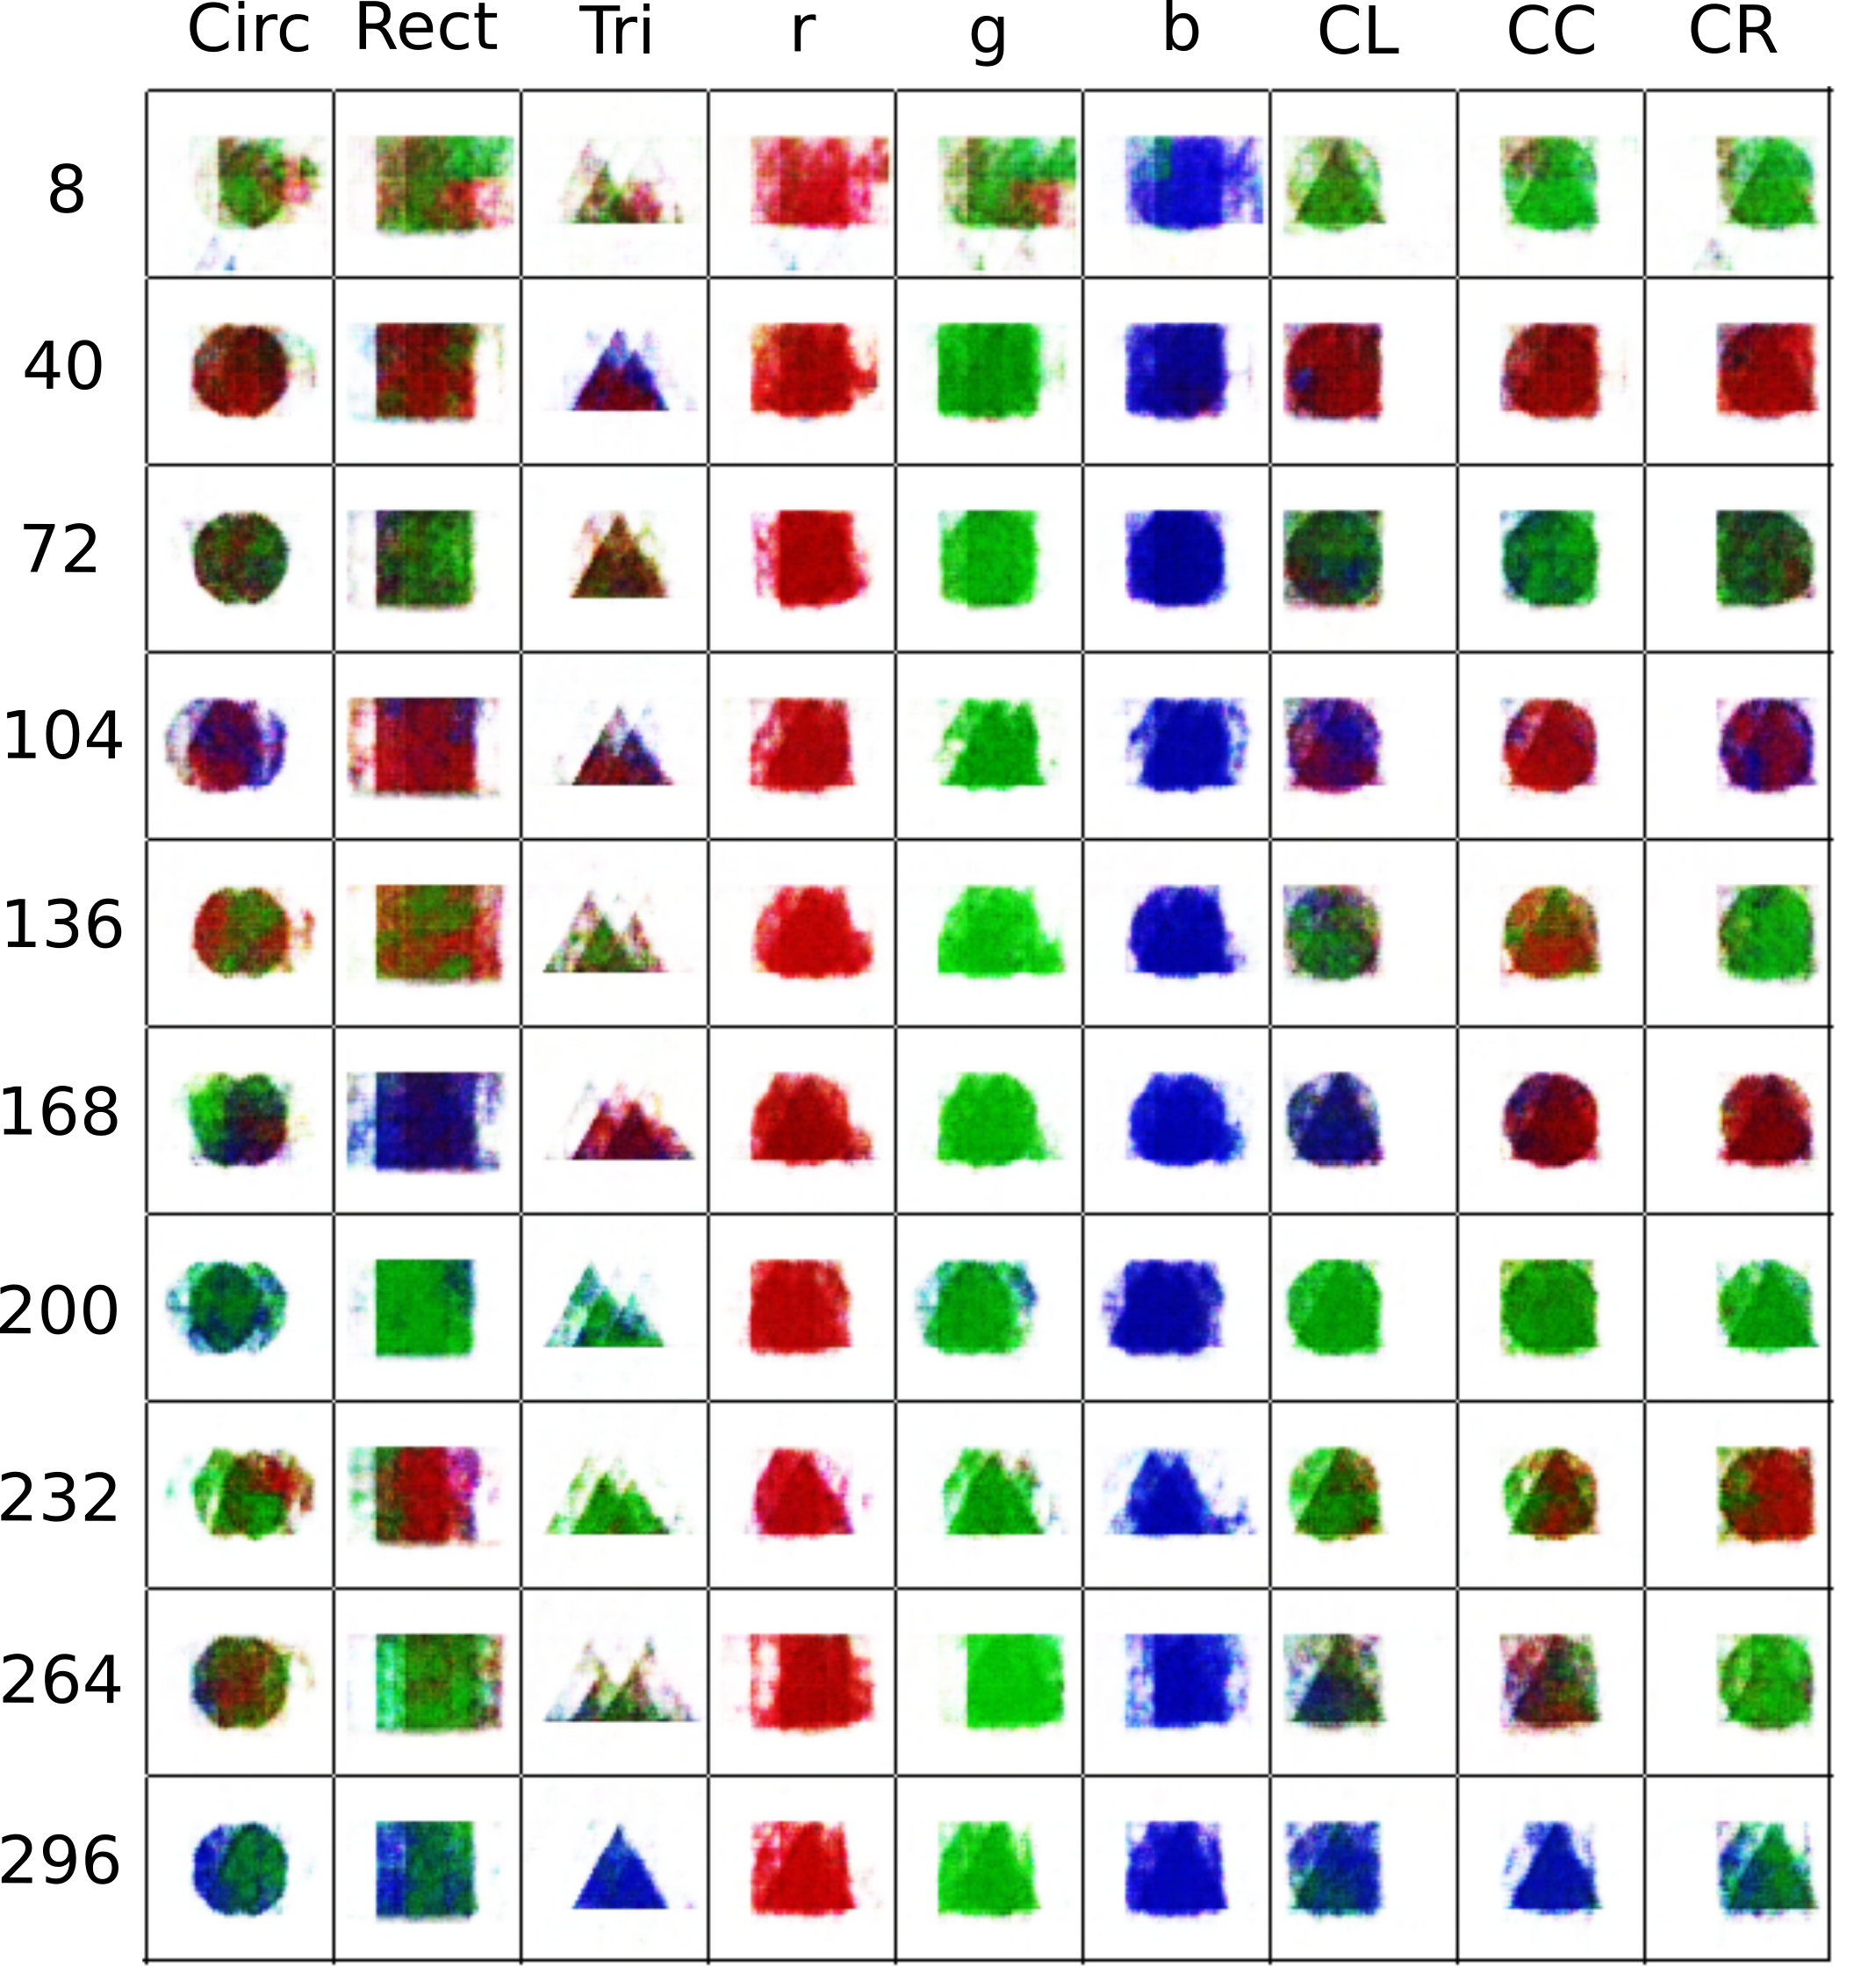
\includegraphics[width=0.75\textwidth]{Figs/shapes/singlelabel331A.png}
\caption{Images generated of each word for different sizes of embedding using the MAE trained in experiment 1 run A.}
\label{fig:331singleA}
\end{figure}
\begin{figure}
\centering
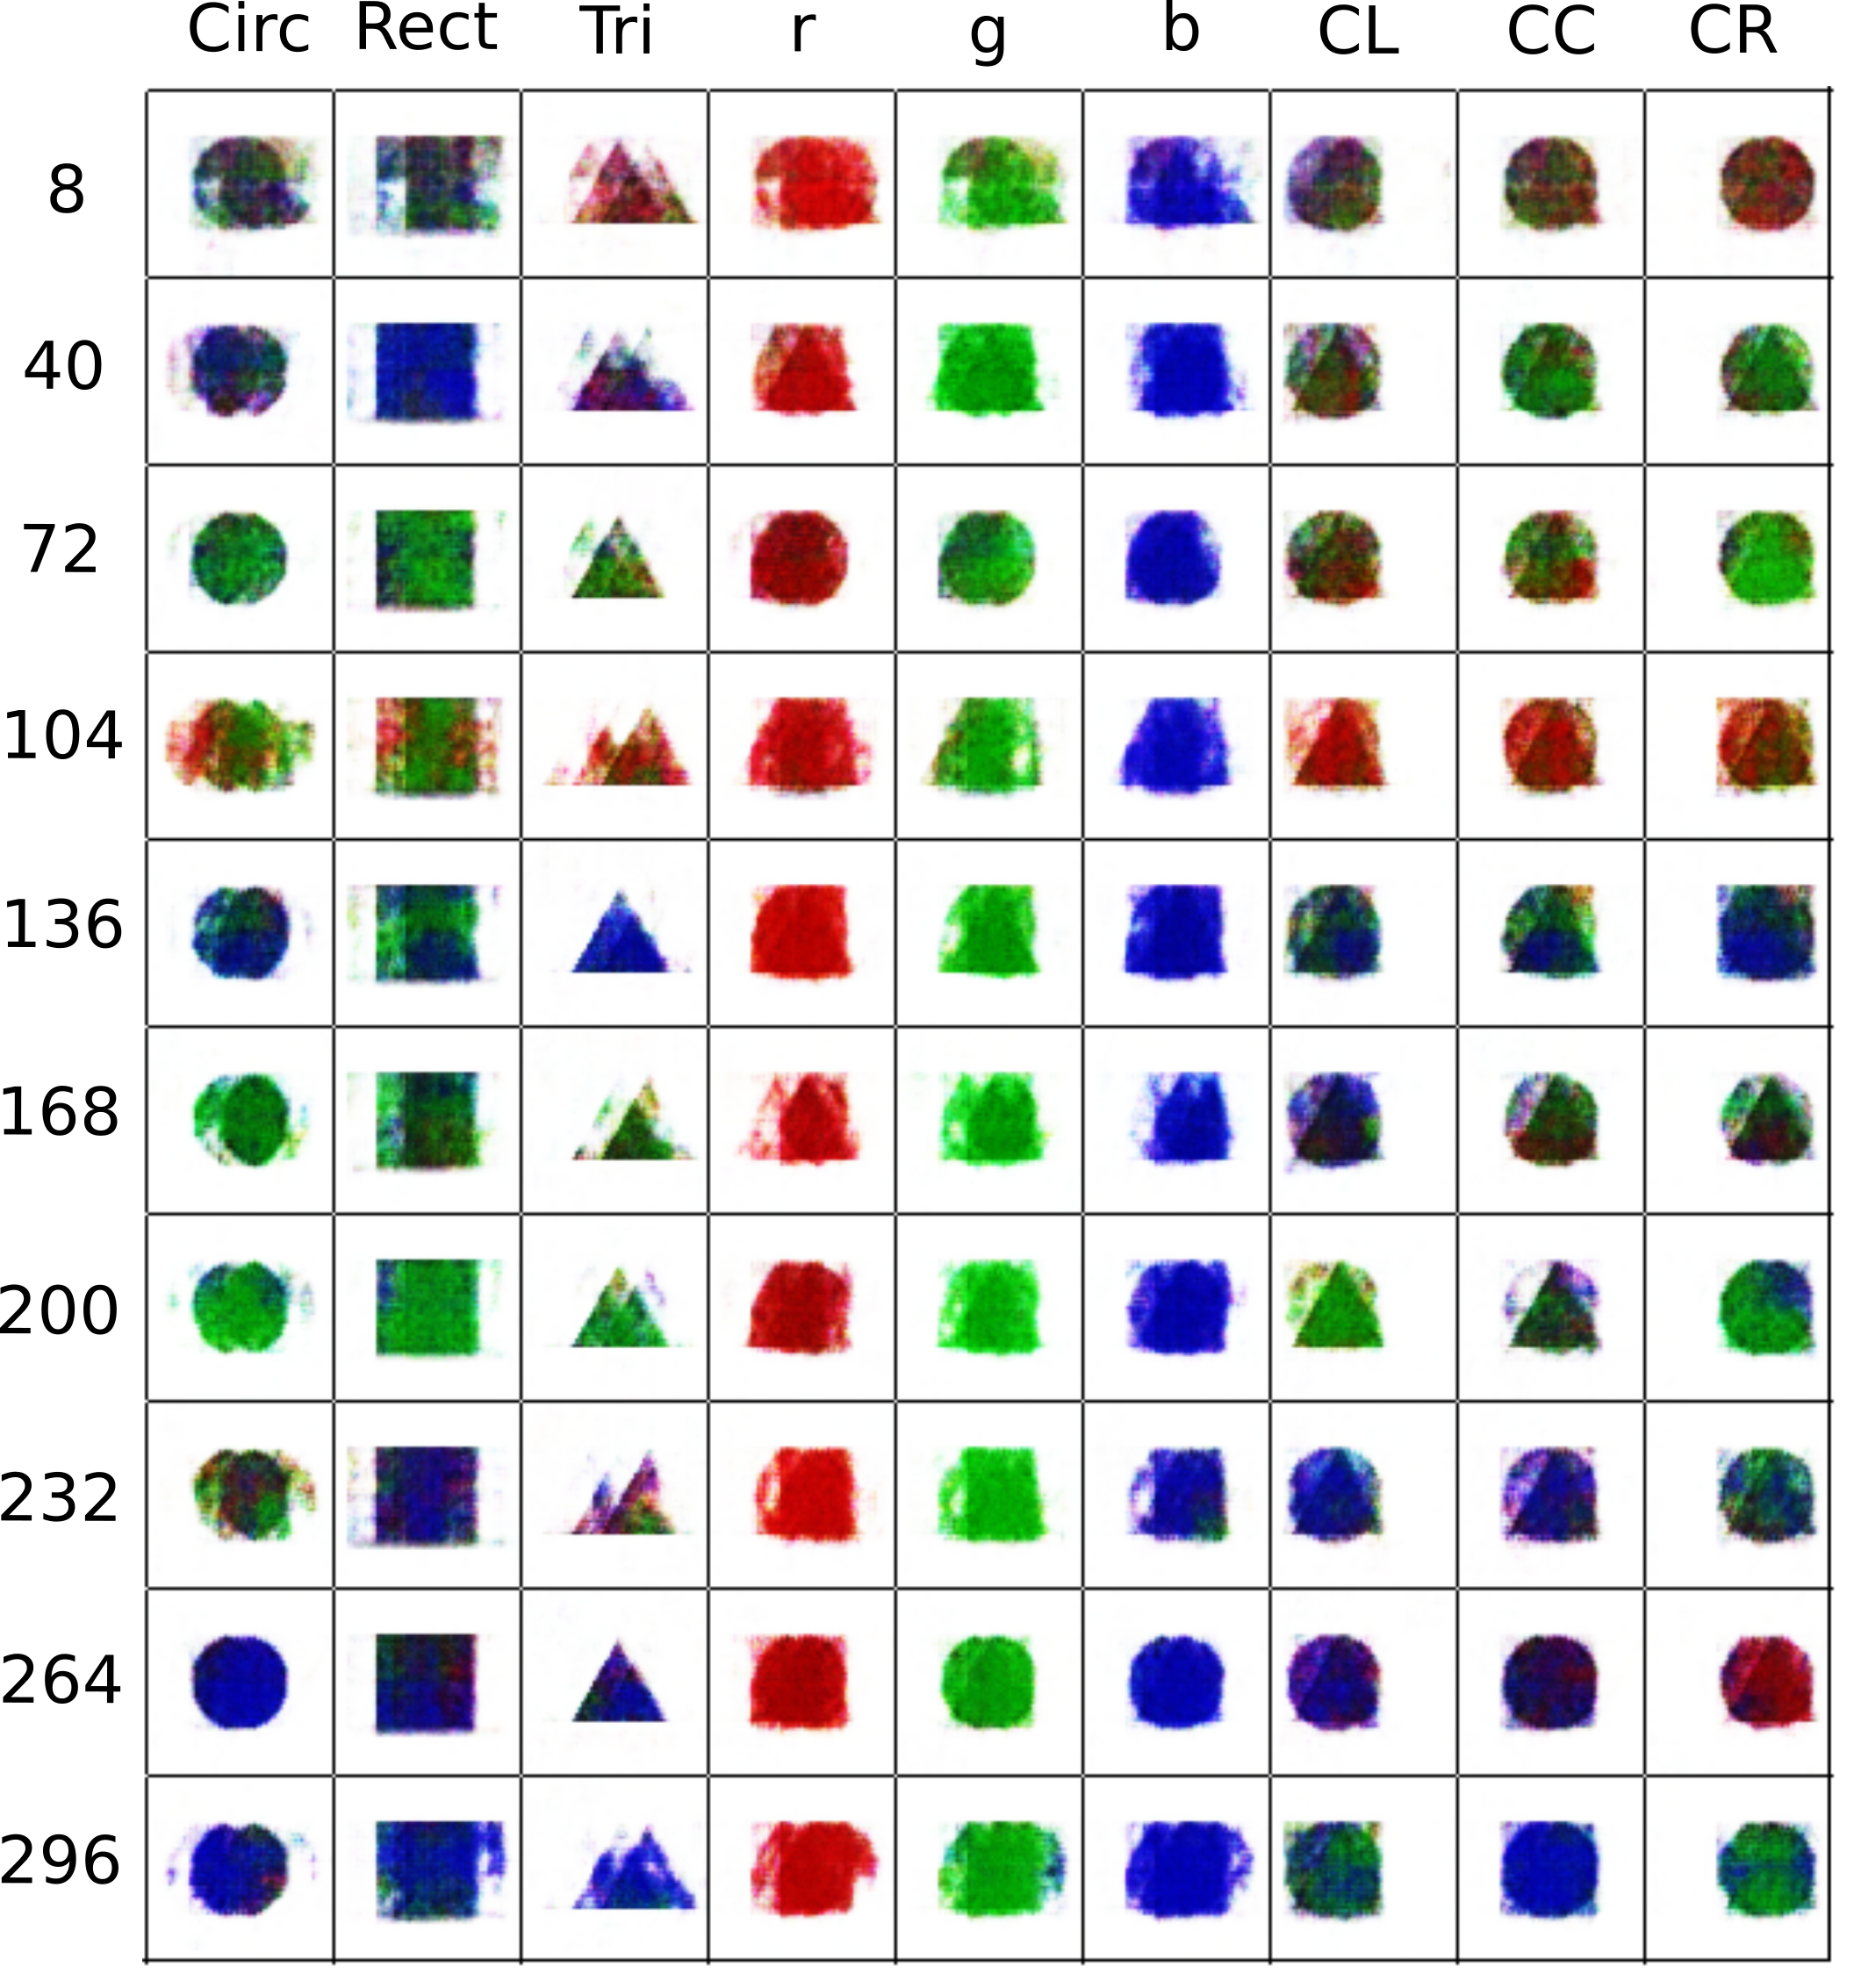
\includegraphics[width=0.75\textwidth]{Figs/shapes/singlelabel331B.png}
\caption{Images generated of each word for different sizes of embedding using the MAE trained in experiment 1 run B.}
\label{fig:331singleB}
\end{figure}
\begin{figure}
\centering
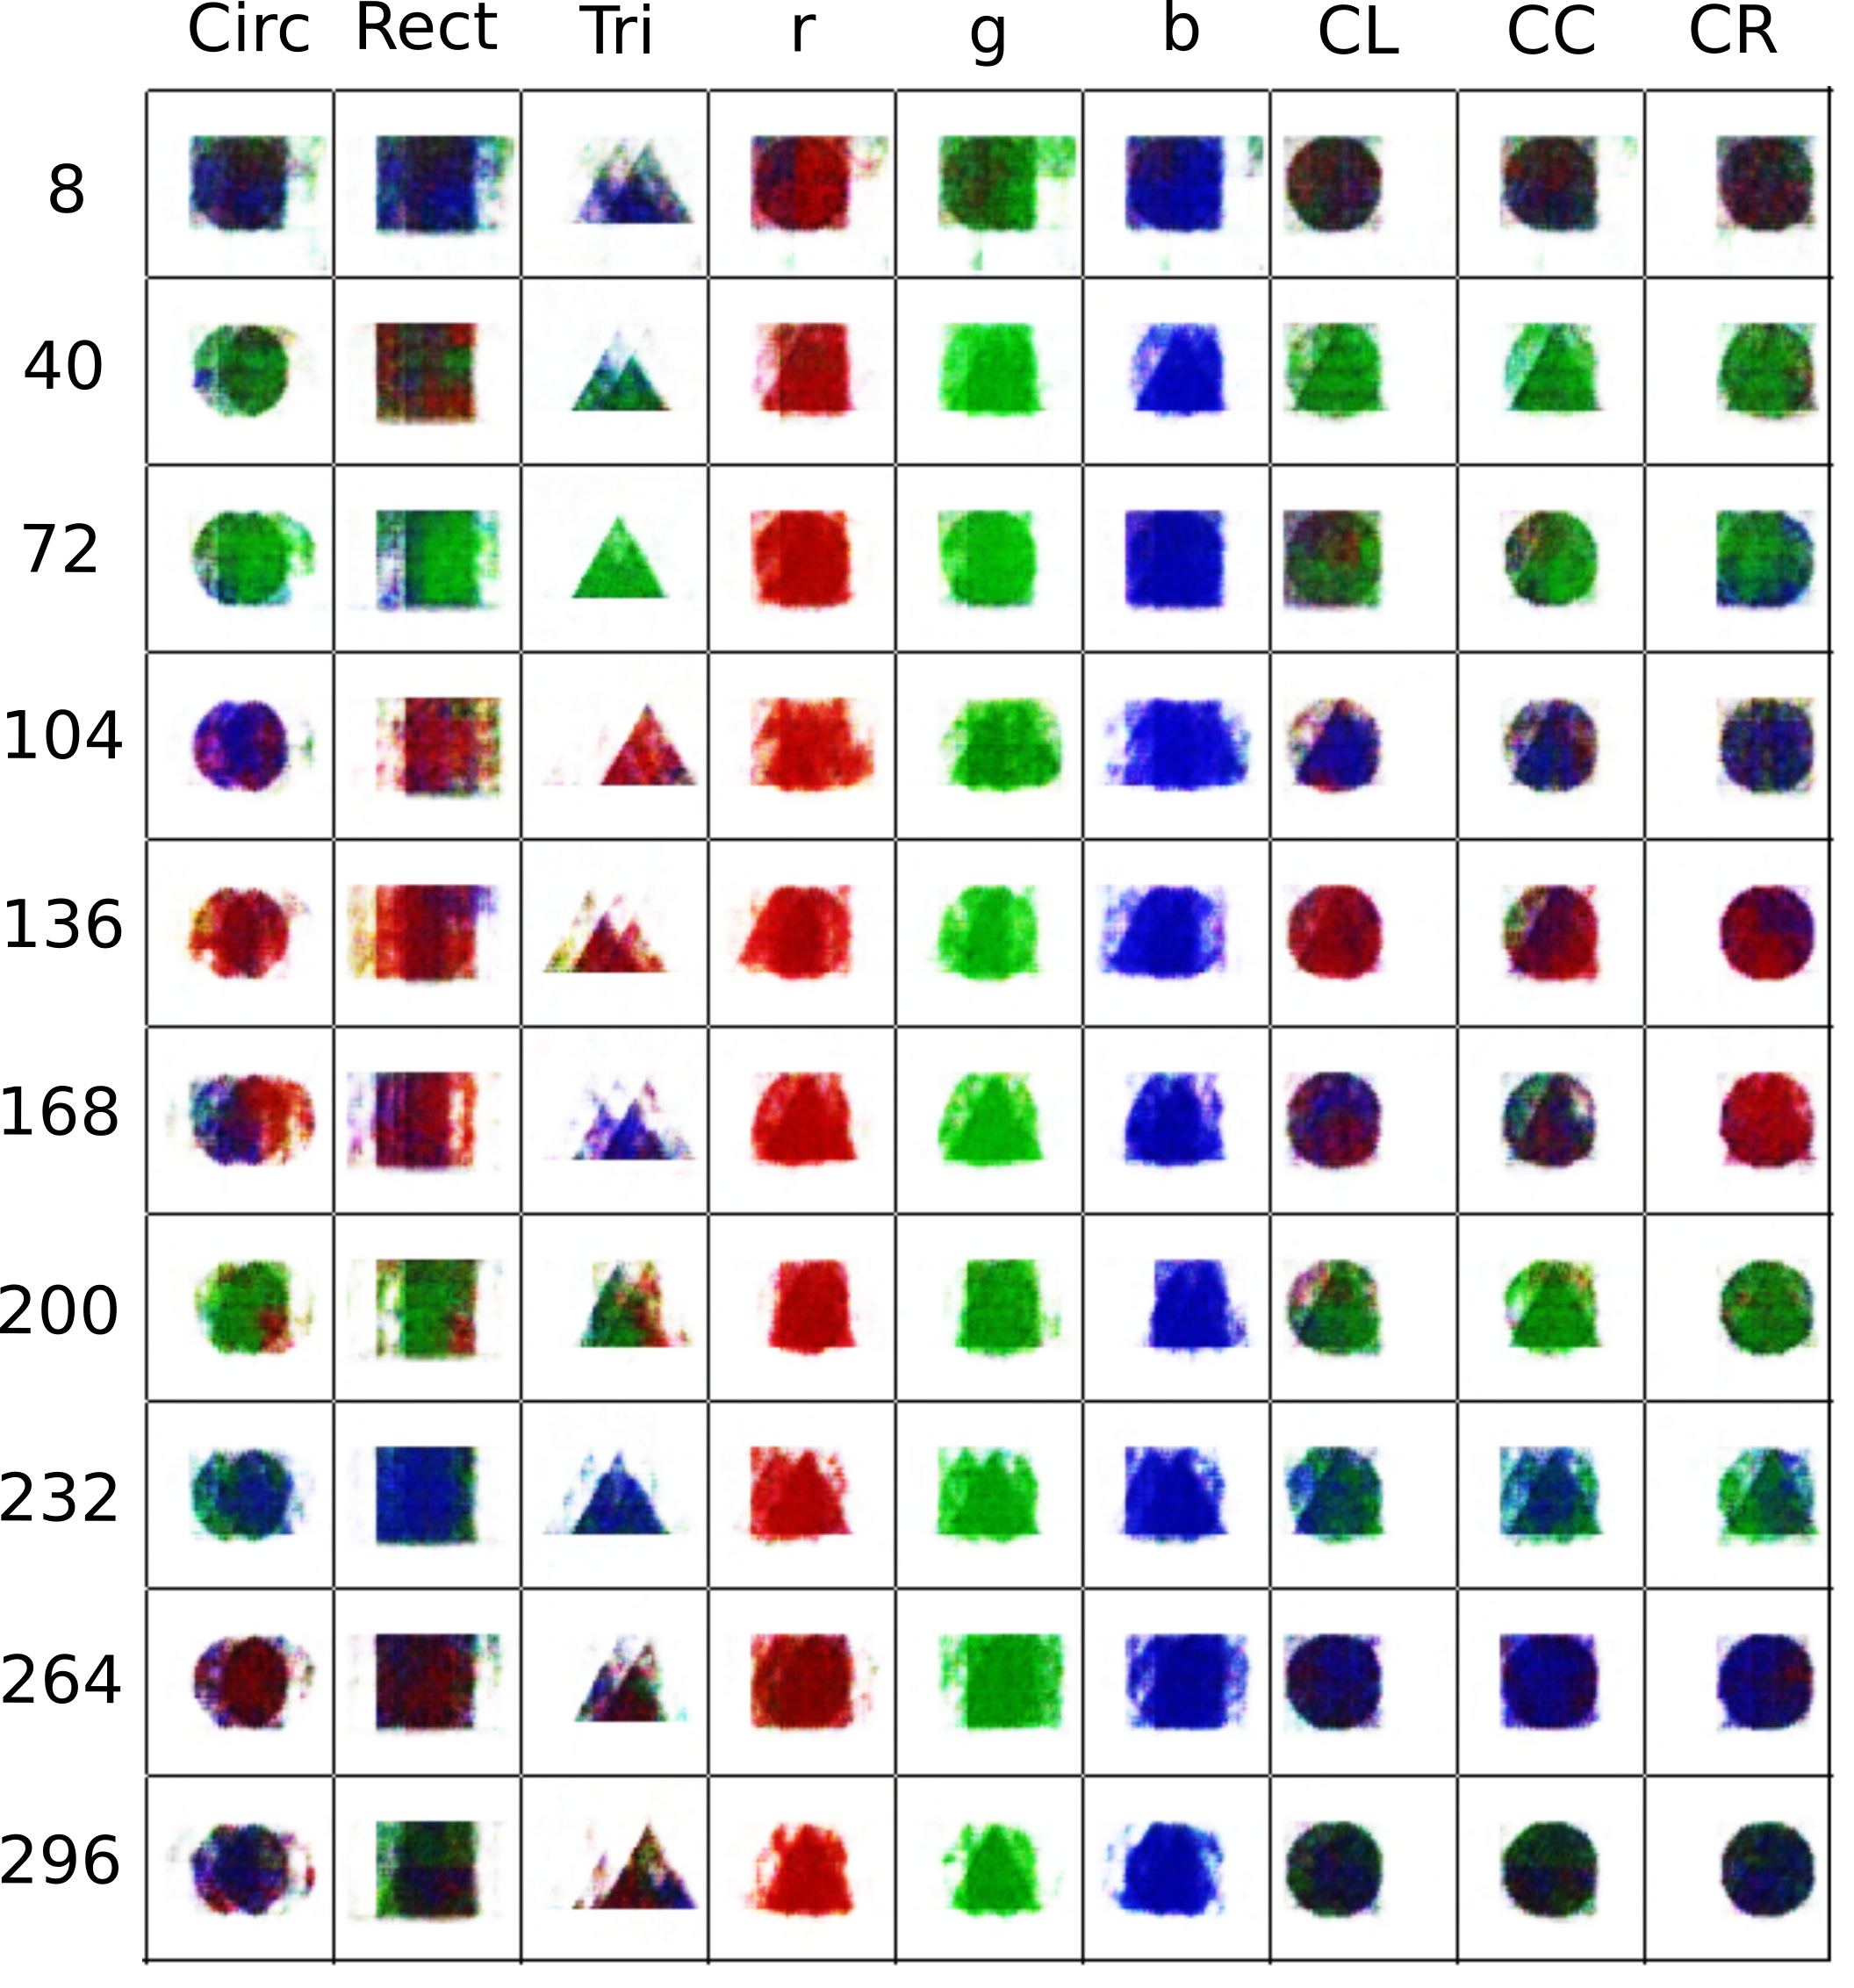
\includegraphics[width=0.75\textwidth]{Figs/shapes/singlelabel331C.png}
\caption{Images generated of each word for different sizes of embedding using the MAE trained in experiment 1 run C.}
\label{fig:331singleC}
\end{figure}
\begin{figure}
\centering
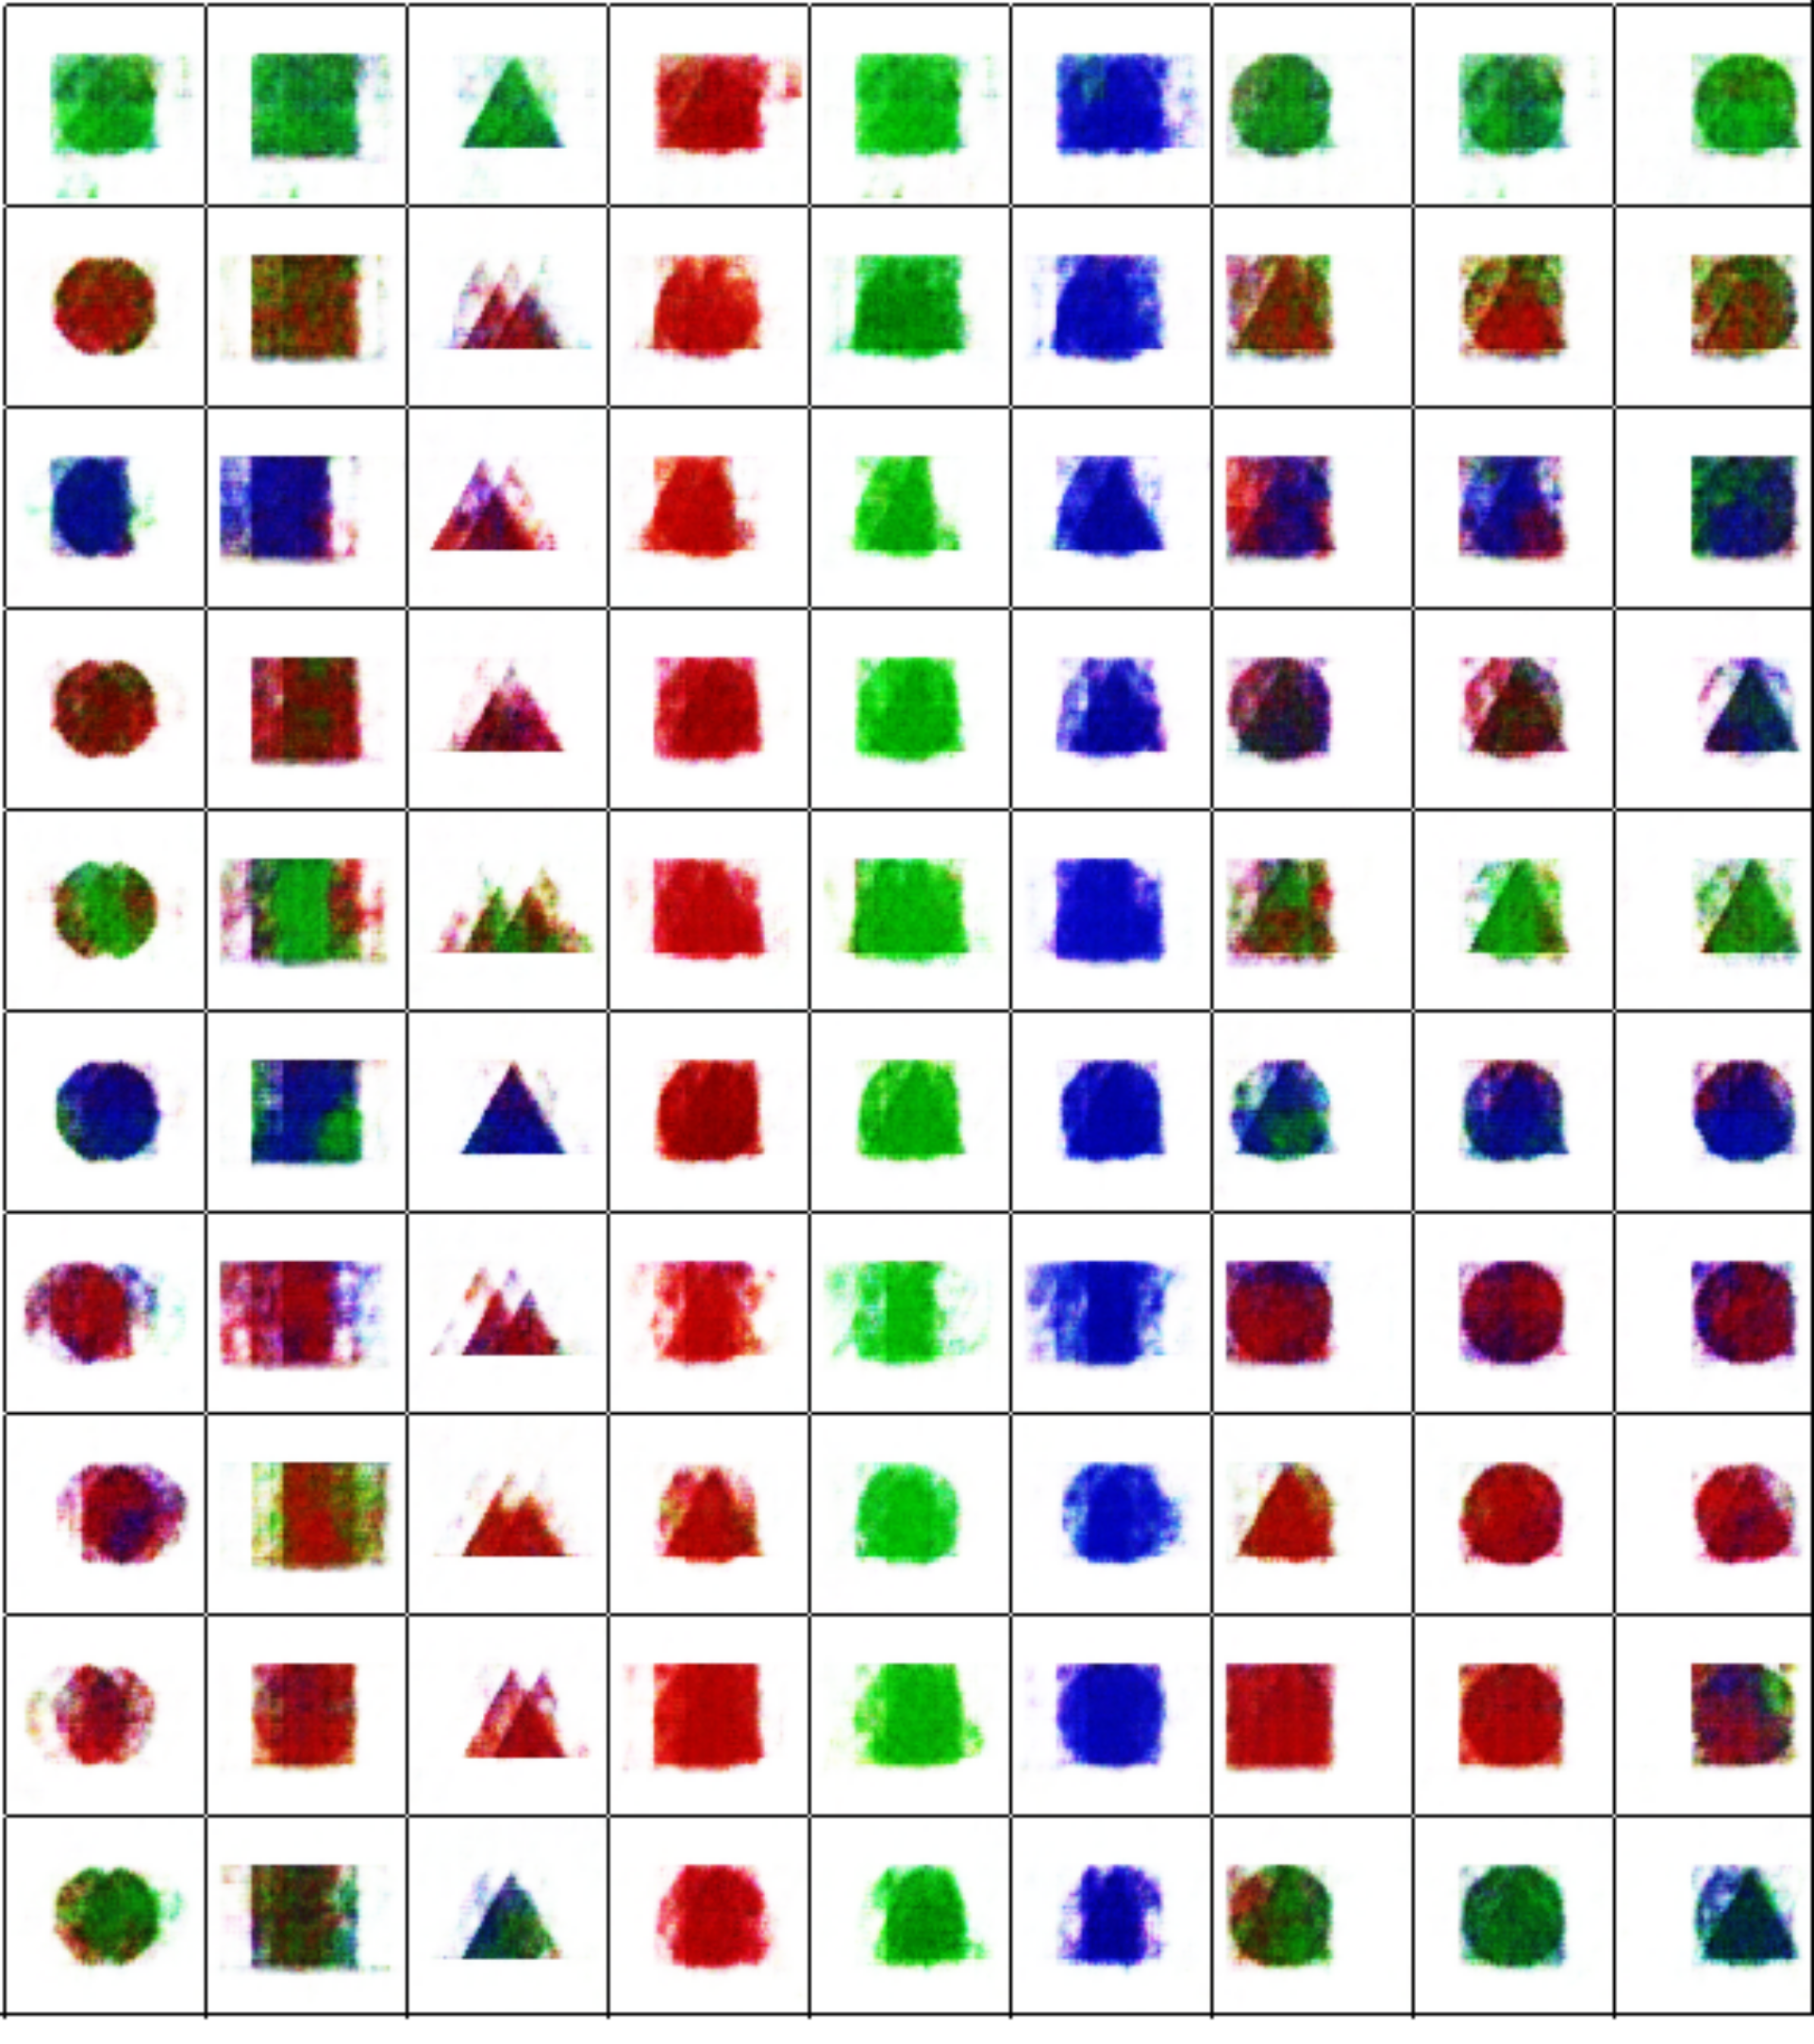
\includegraphics[width=0.75\textwidth]{Figs/shapes/singlelabel331D.png}
\caption{Images generated of each word for different sizes of embedding using the MAE trained in experiment 1 run D.}
\label{fig:331singleD}
\end{figure}


\begin{figure}
\centering
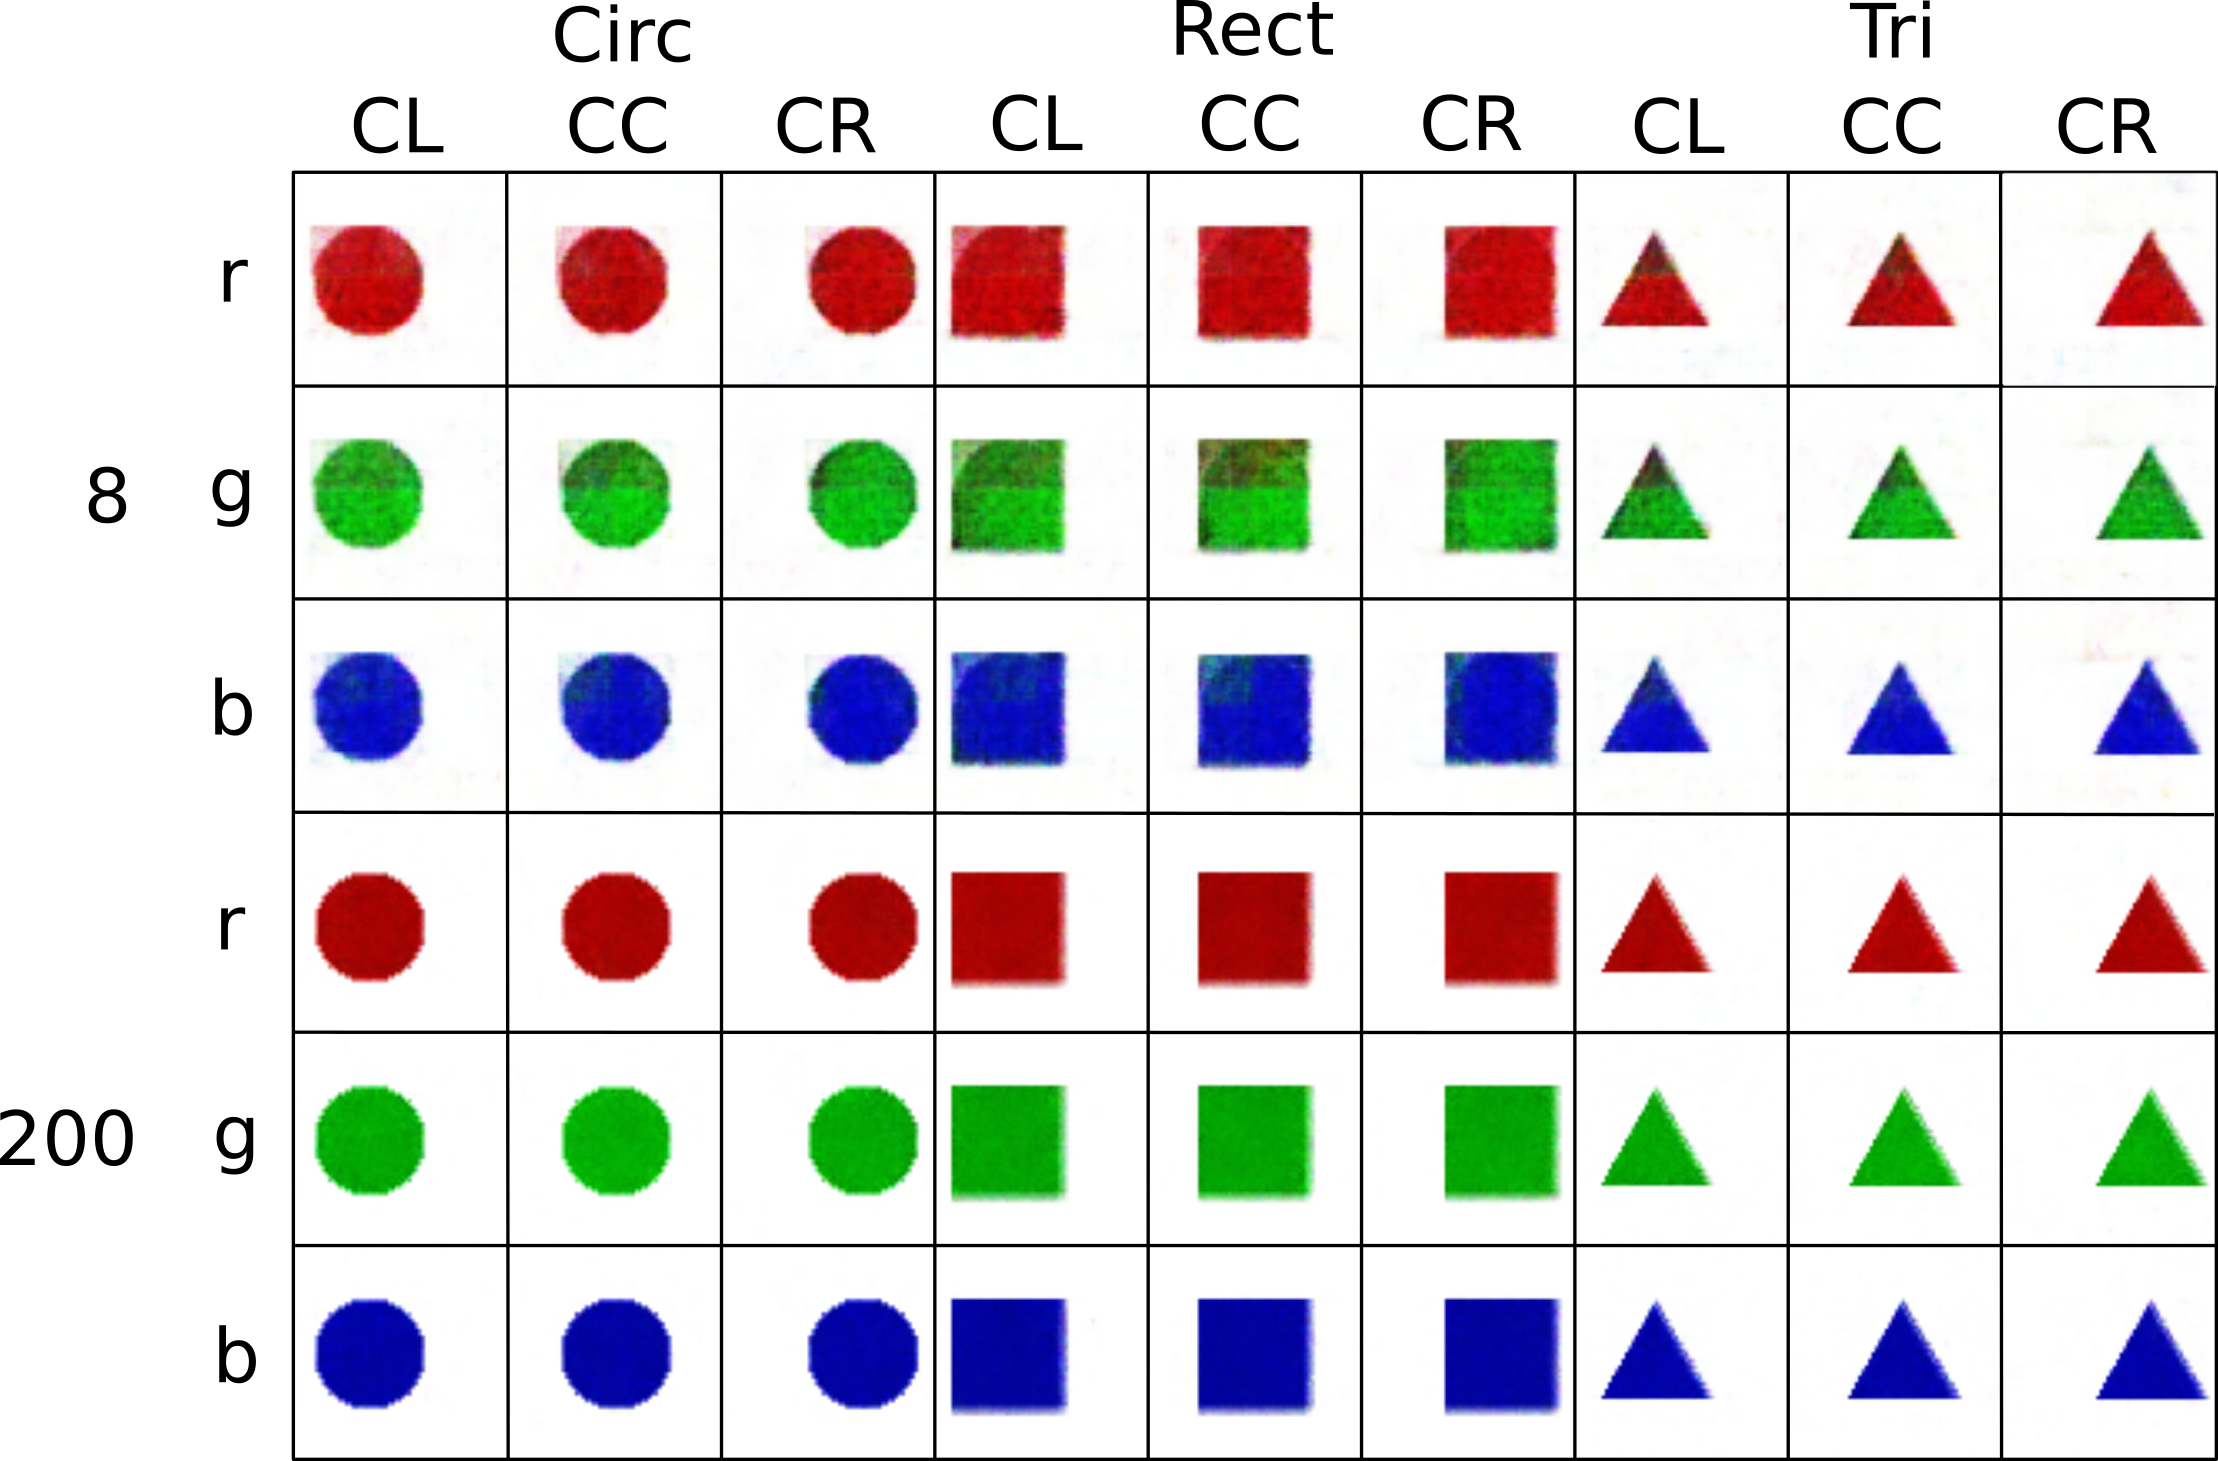
\includegraphics[width=0.75\textwidth]{Figs/shapes/331_8v200.png}
\caption{Images generated from descriptions with an embedding size of 8 or 200.}
\label{fig:8vs200}
\end{figure}


\begin{figure}
\centering
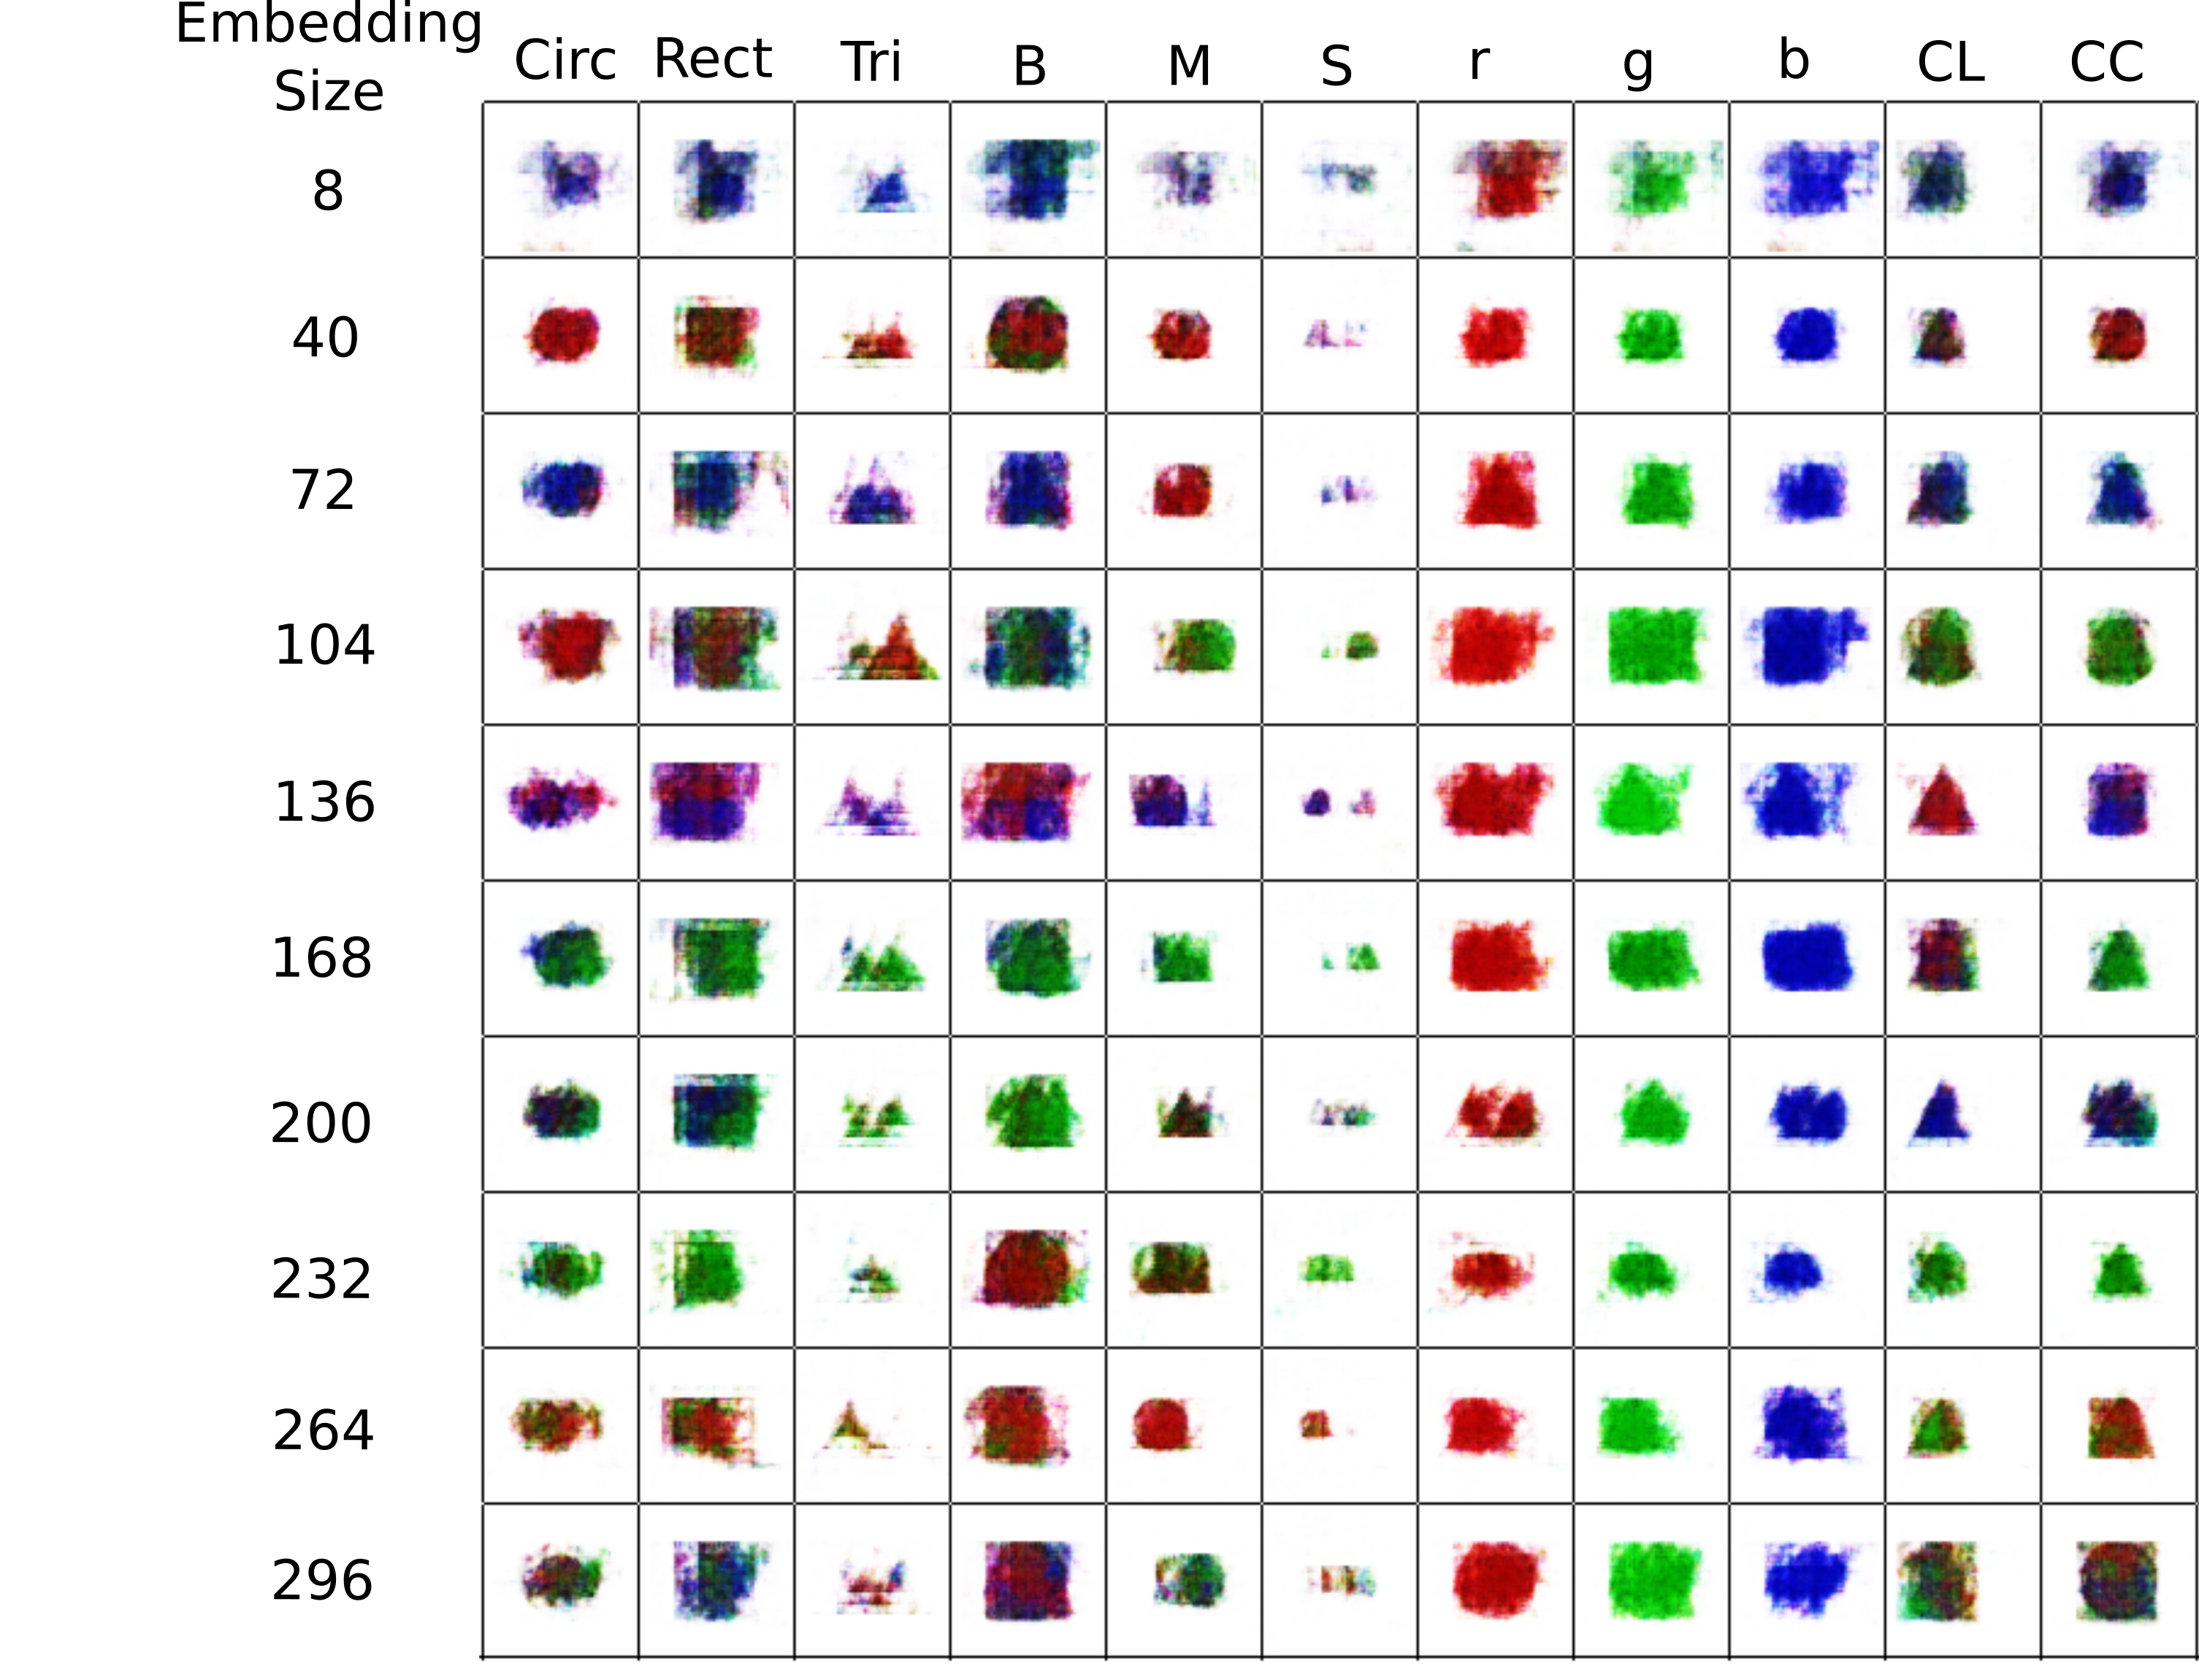
\includegraphics[width=0.75\textwidth]{Figs/shapes/singlelabel333A.png}
\caption{Images generated of each word for different sizes of embedding using the MAE trained in experiment 2 run A.}
\label{fig:333singleA}
\end{figure}
\begin{figure}
\centering
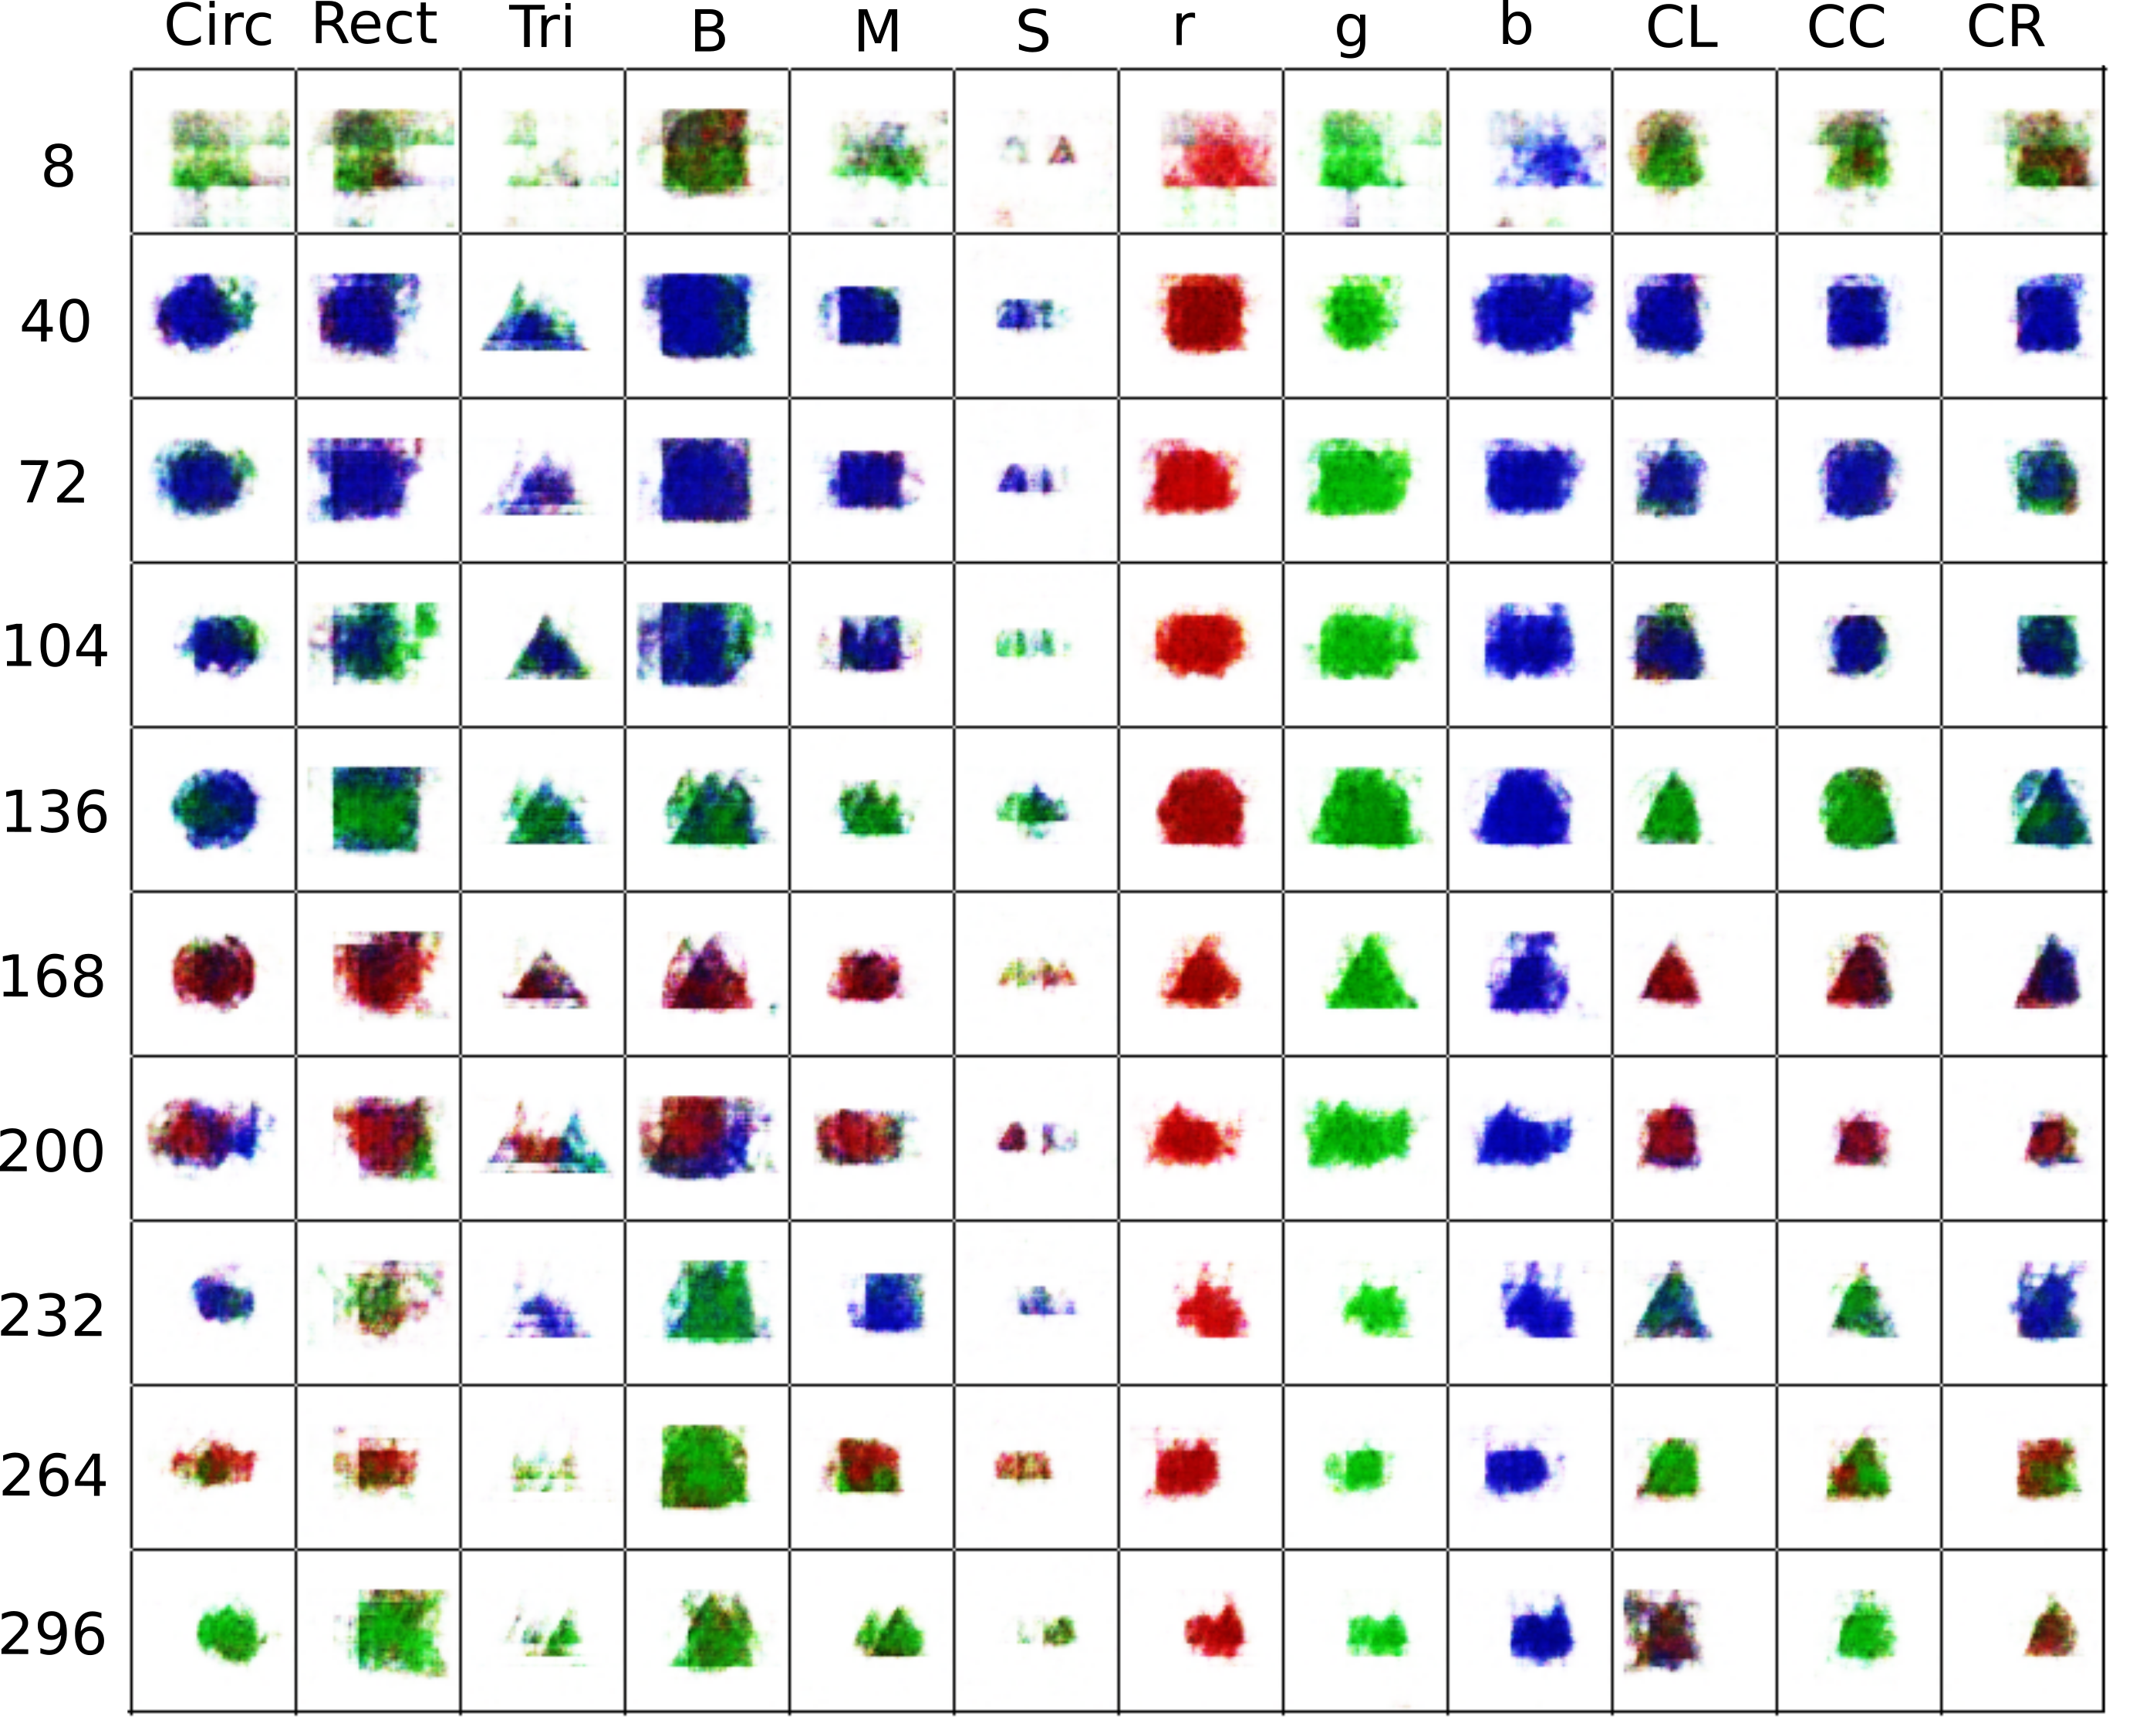
\includegraphics[width=0.75\textwidth]{Figs/shapes/singlelabel333B.png}
\caption{Images generated of each word for different sizes of embedding using the MAE trained in experiment 2 run B.}
\label{fig:333singleB}
\end{figure}
\begin{figure}
\centering
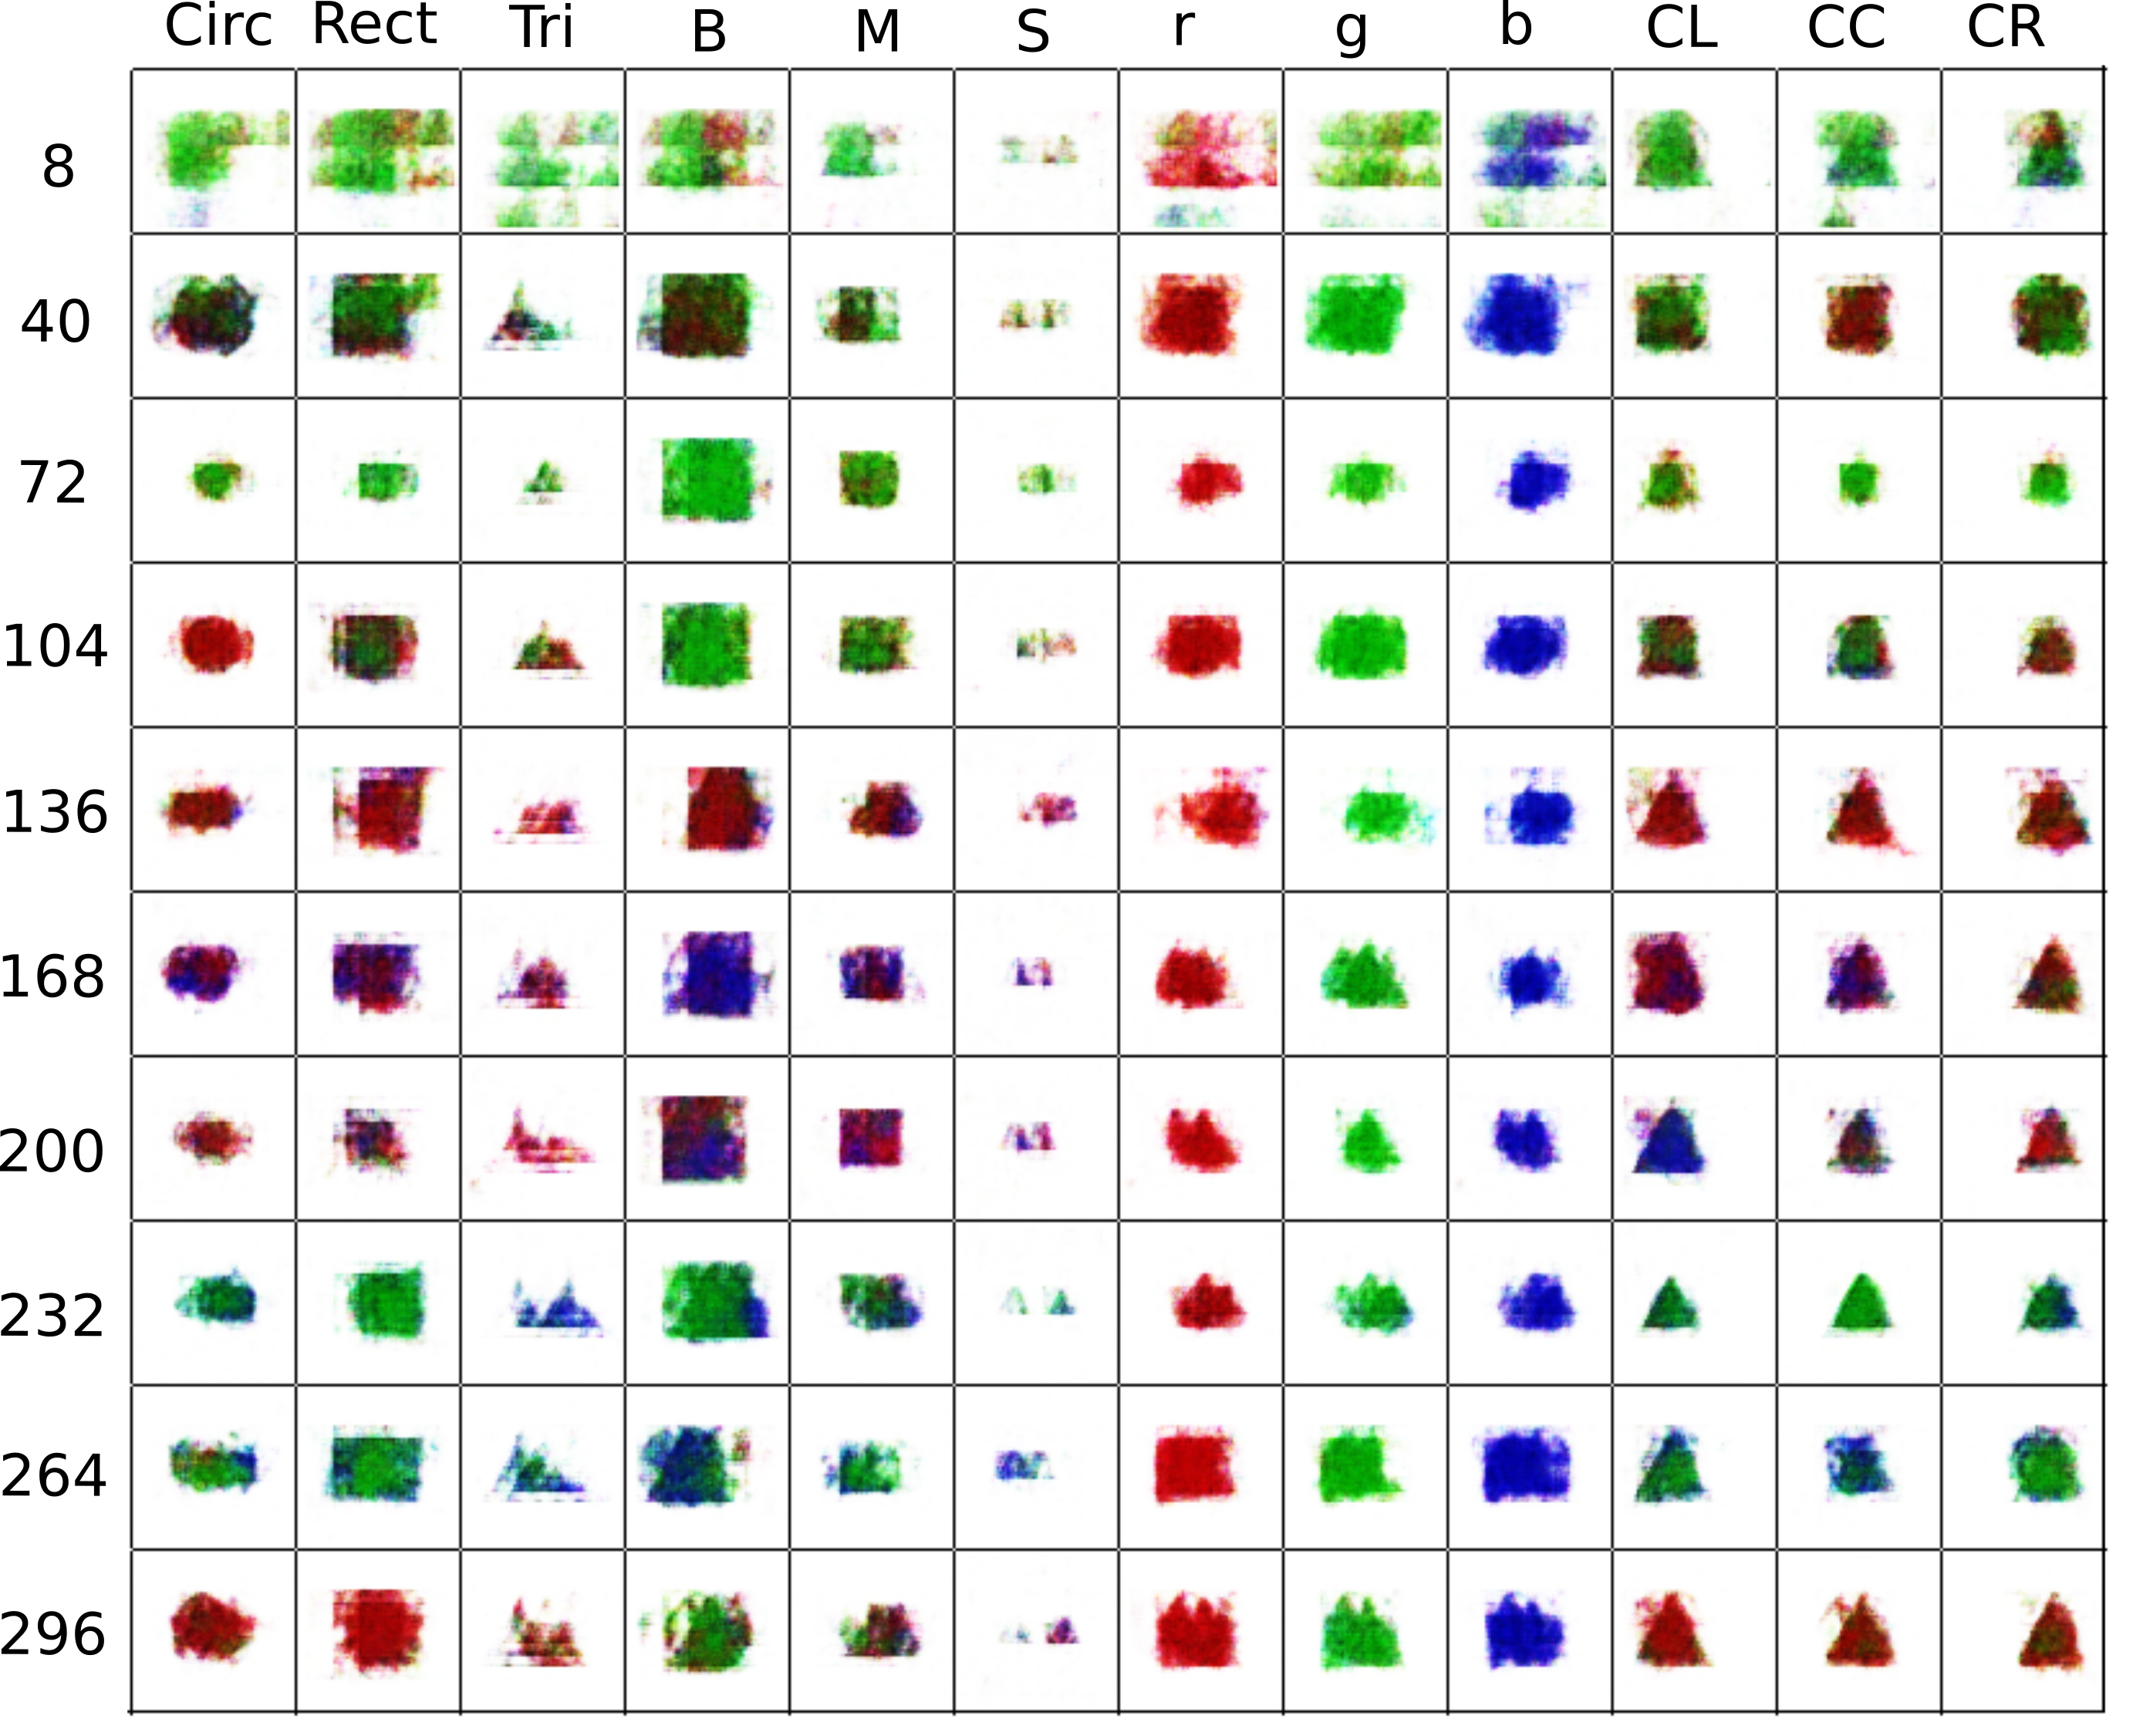
\includegraphics[width=0.75\textwidth]{Figs/shapes/singlelabel333C.png}
\caption{Images generated of each word for different sizes of embedding using the MAE trained in experiment 2 run C.}
\label{fig:333singleC}
\end{figure}
\begin{figure}
\centering
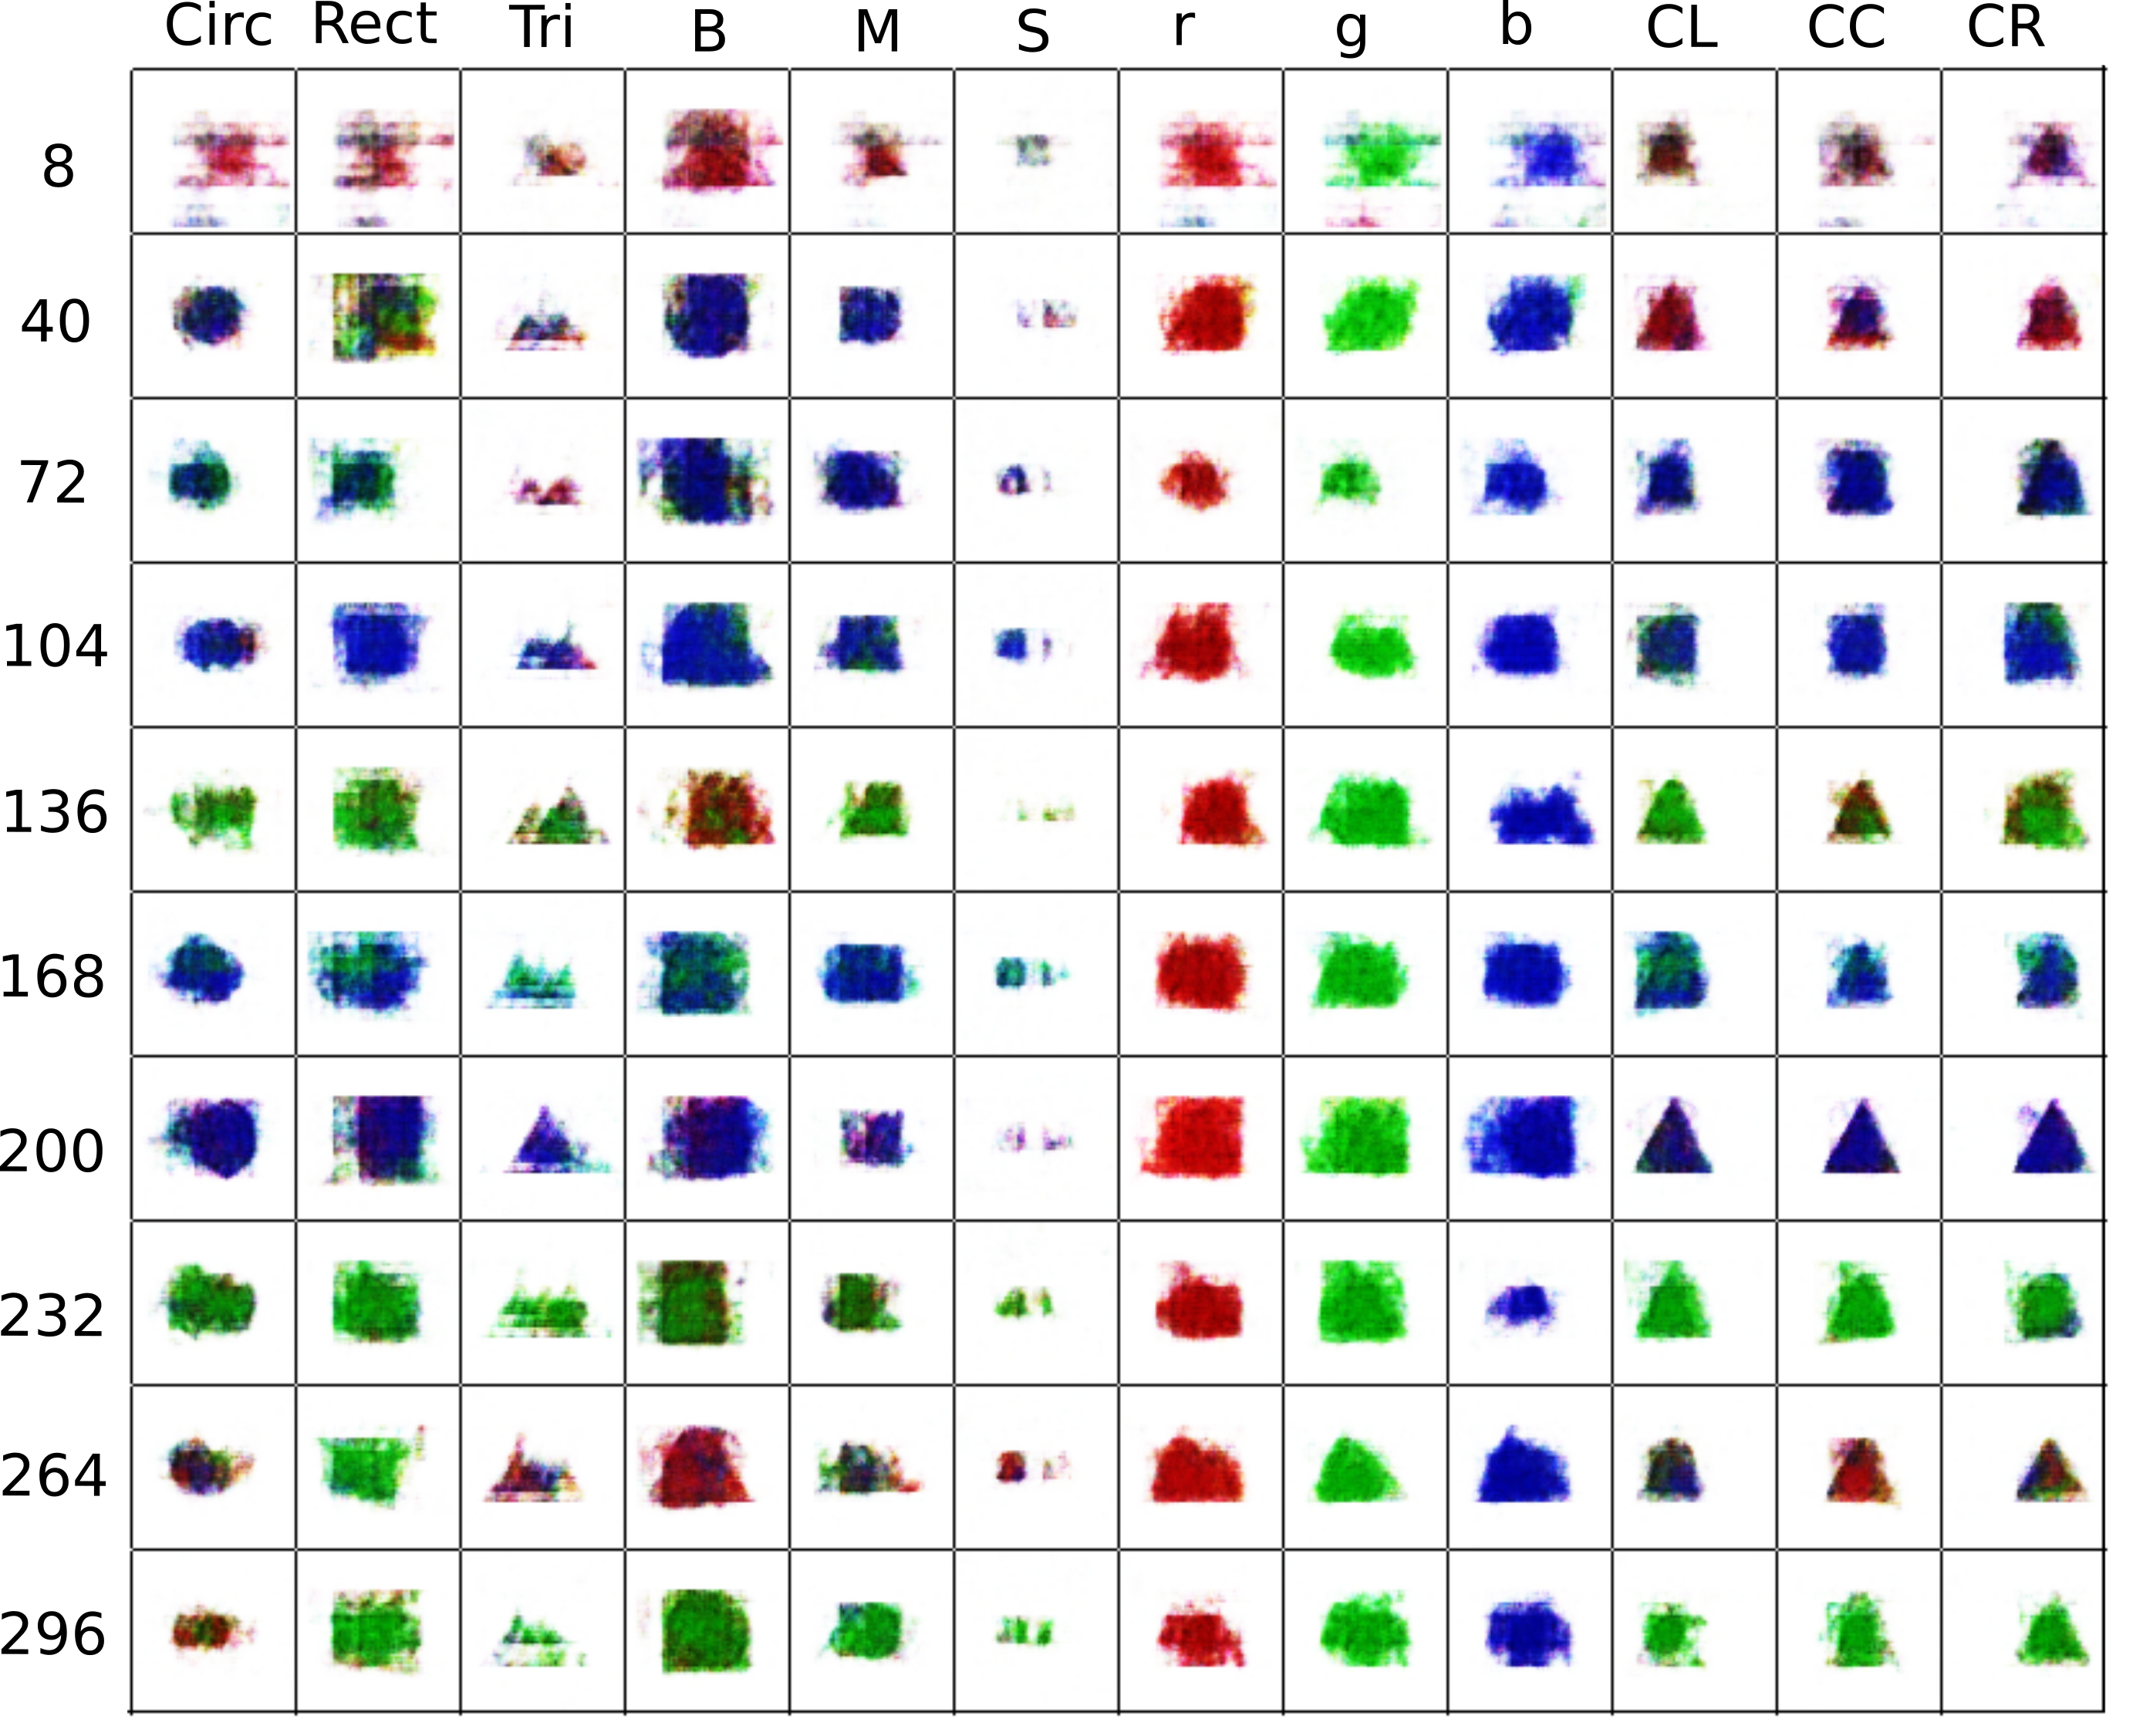
\includegraphics[width=0.75\textwidth]{Figs/shapes/singlelabel333D.png}
\caption{Images generated of each word for different sizes of embedding using the MAE trained in experiment 2 run D.}
\label{fig:333singleD}
\end{figure}

\begin{figure}
\centering
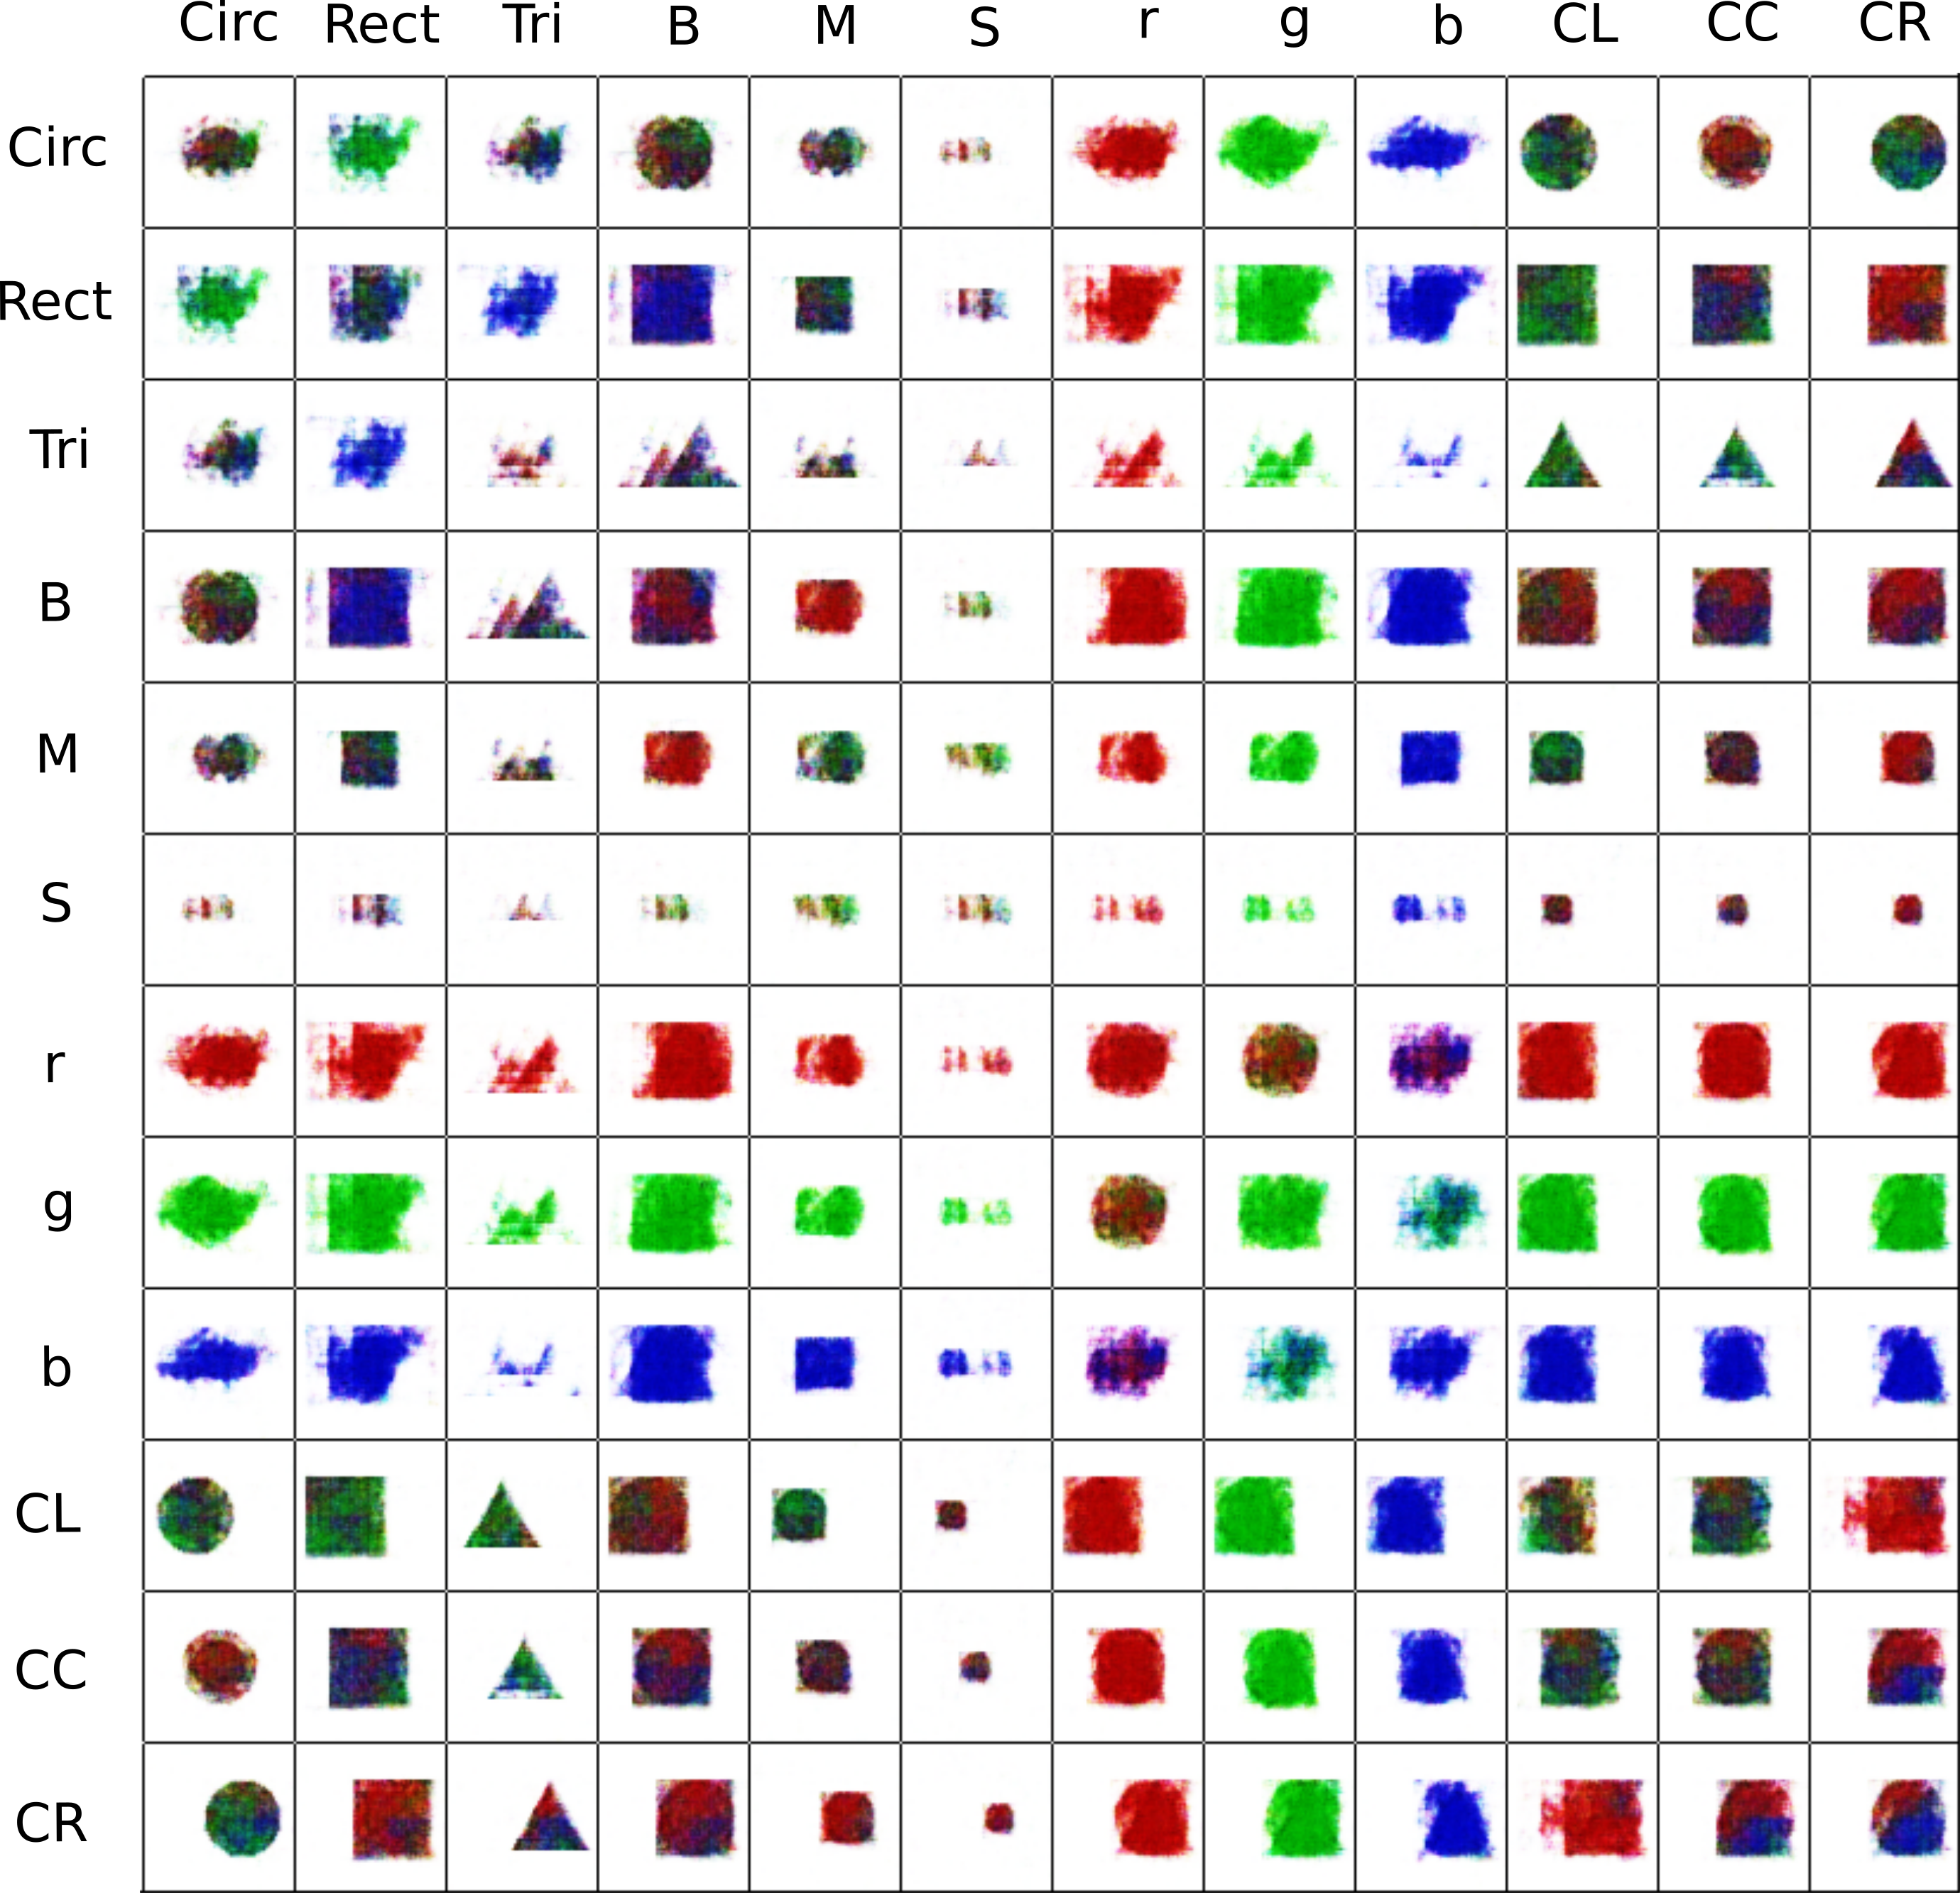
\includegraphics[width=0.75\textwidth]{Figs/shapes/2word333A.png}
\caption{Images generated using word pairs using an embedding size of 296 neurons from experiment 2 run A.}
\label{fig:2word333A}
\end{figure}

\begin{figure}
\centering
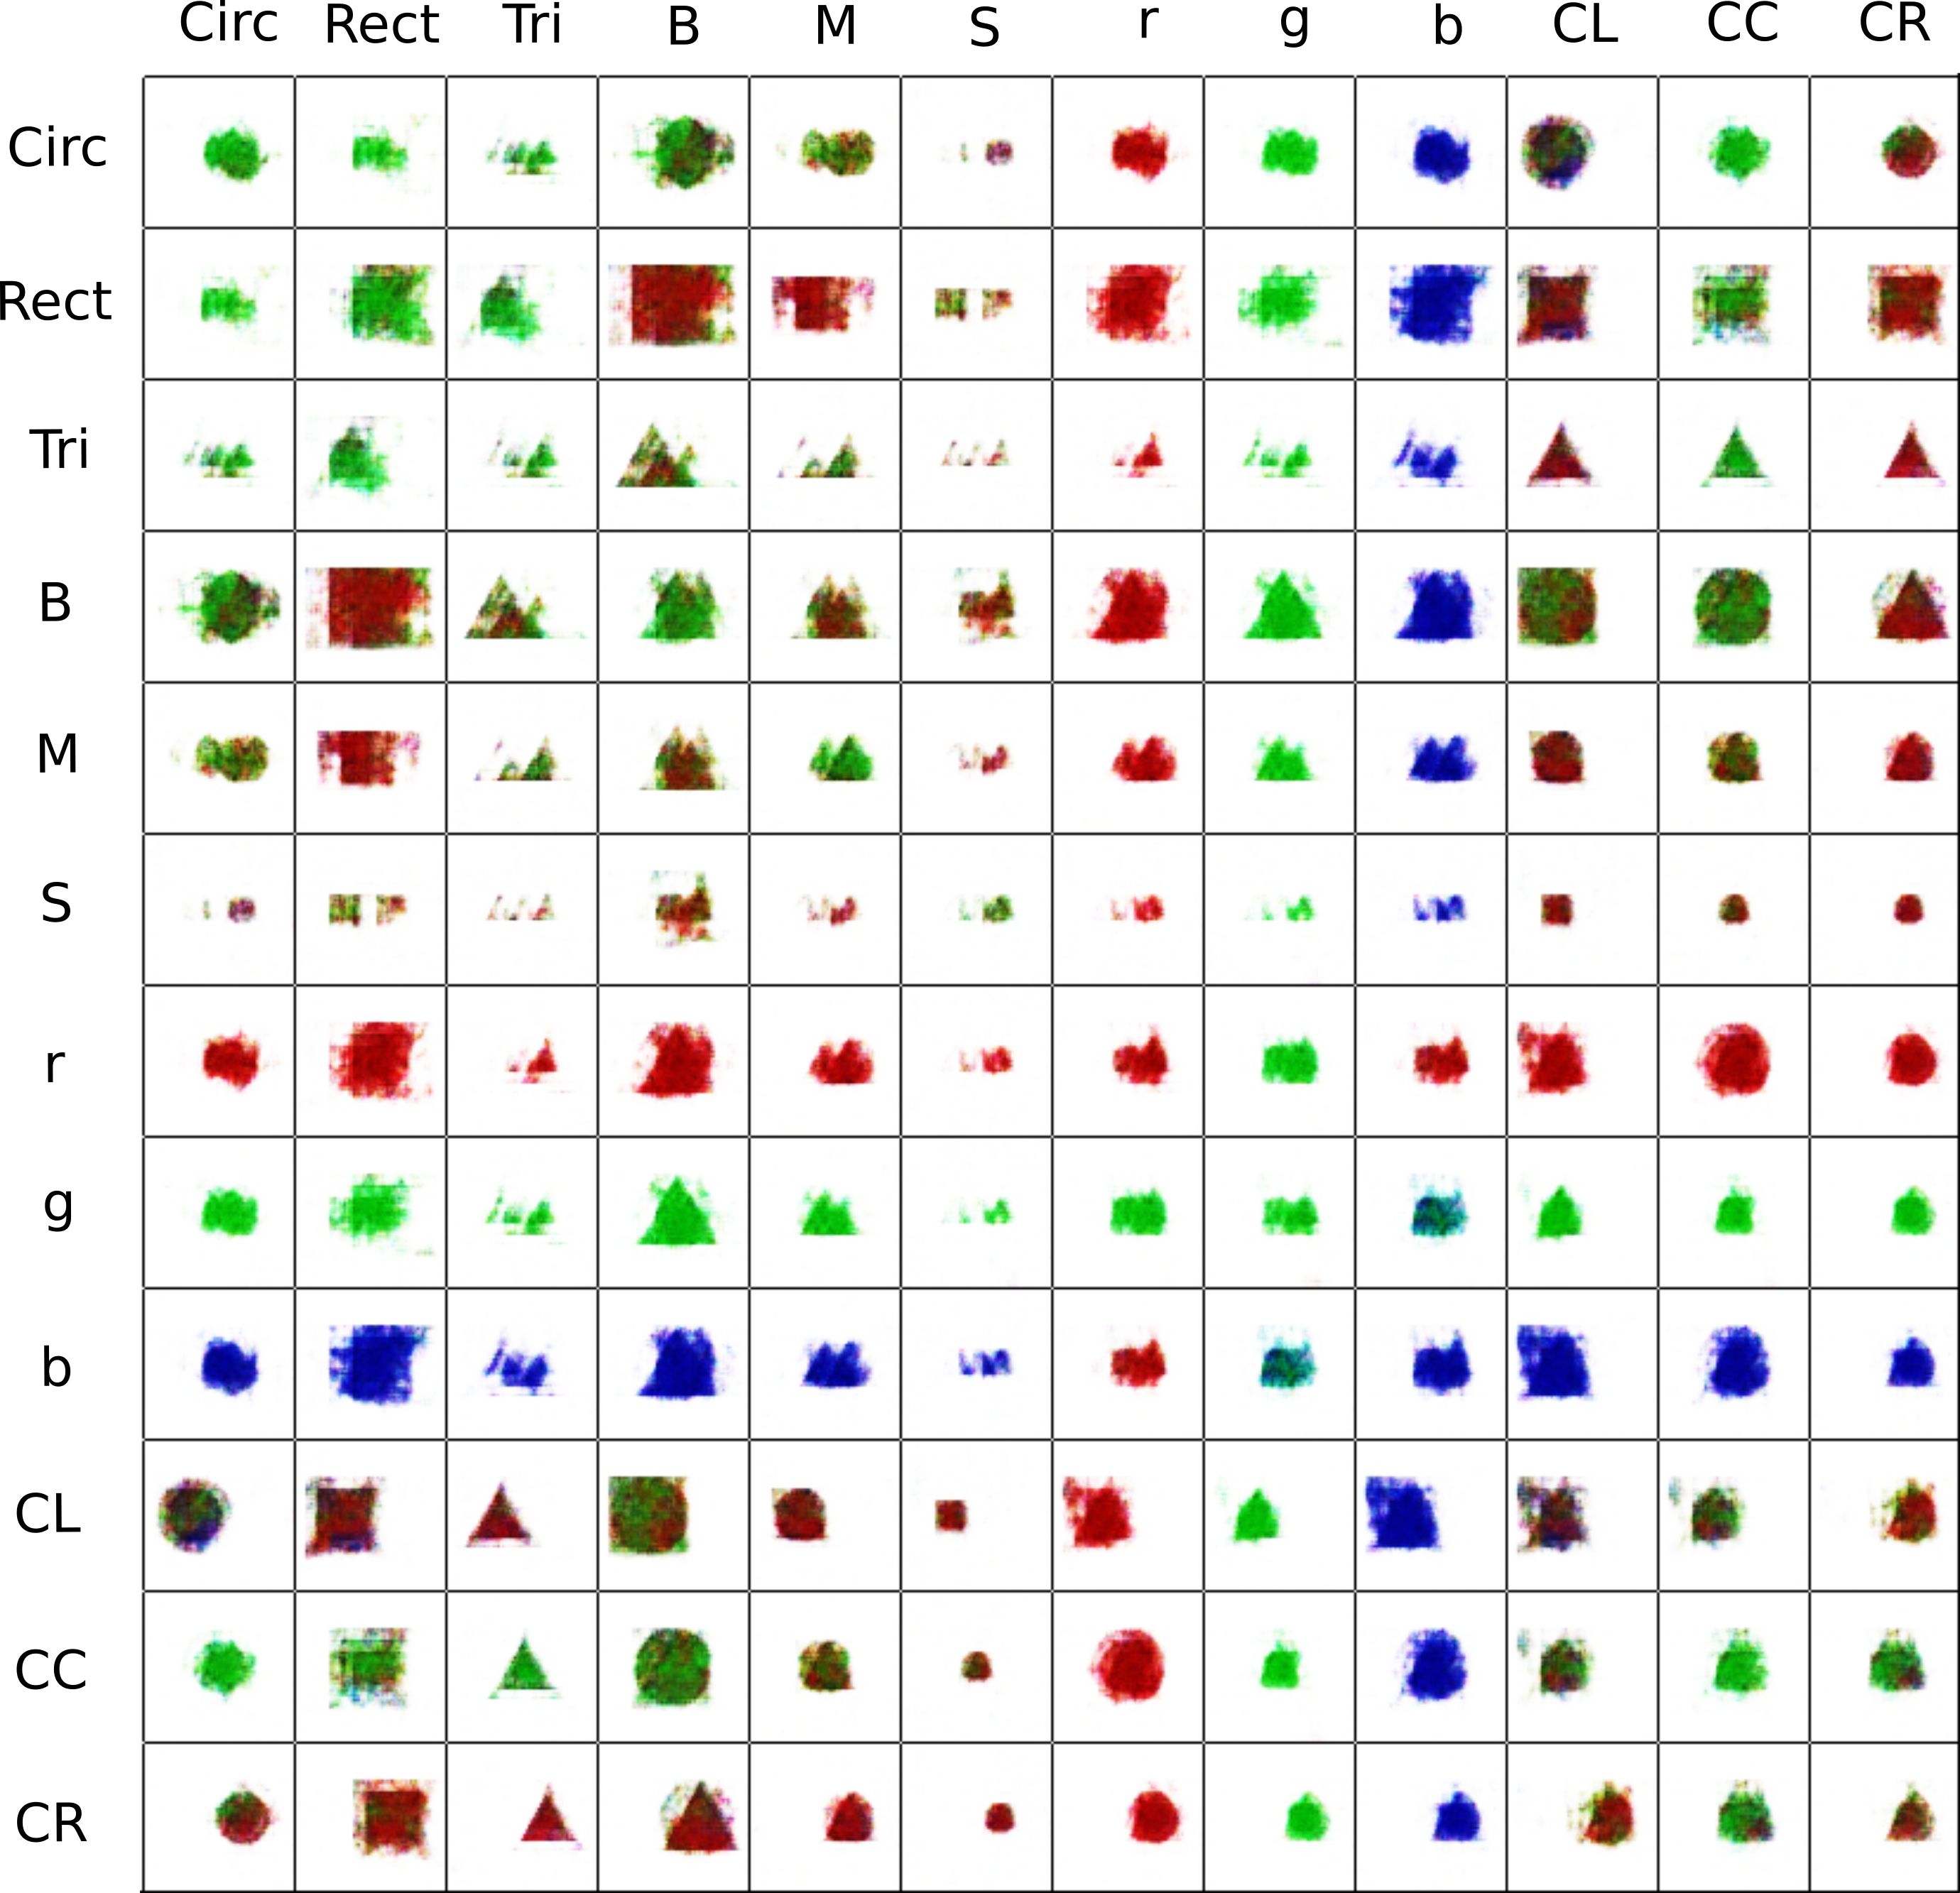
\includegraphics[width=0.75\textwidth]{Figs/shapes/2word333B.png}
\caption{Images generated using word pairs using an embedding size of 296 neurons from experiment 2 run B.}
\label{fig:2word333B}
\end{figure}

\begin{figure}
\centering
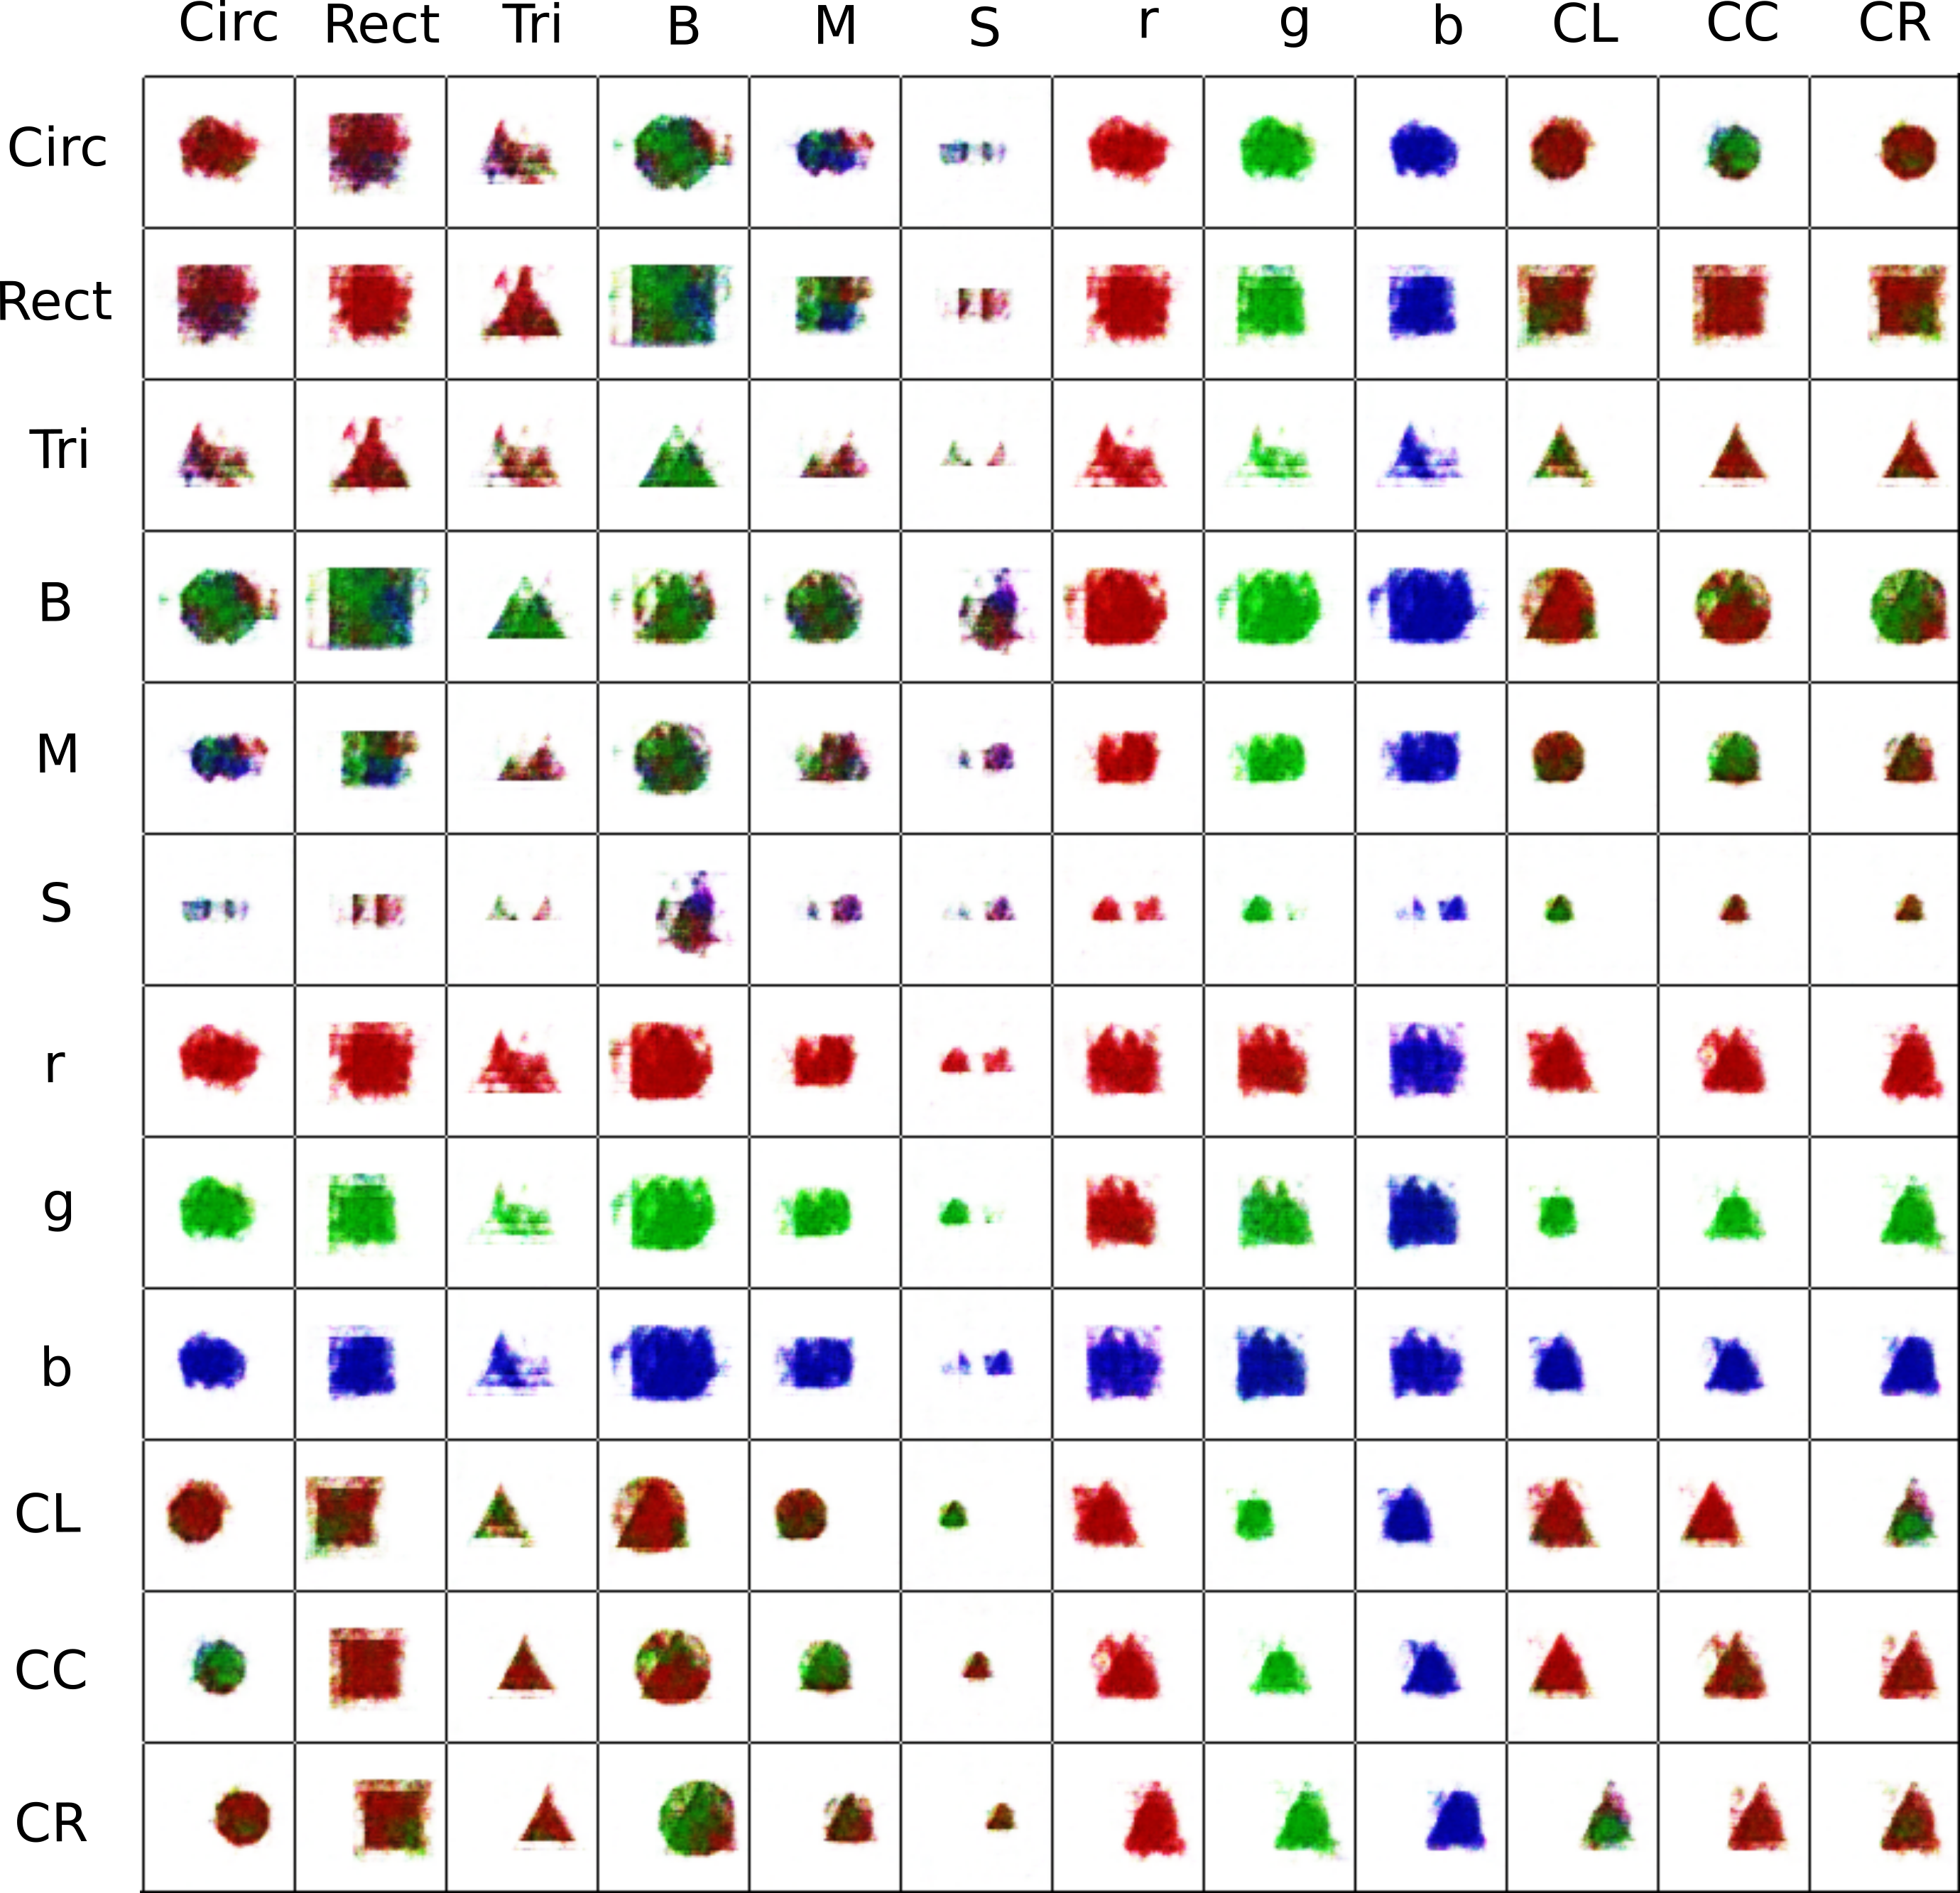
\includegraphics[width=0.75\textwidth]{Figs/shapes/2word333C.png}
\caption{Images generated using word pairs using an embedding size of 296 neurons from experiment 2 run C.}
\label{fig:2word333C}
\end{figure}

\begin{figure}
\centering
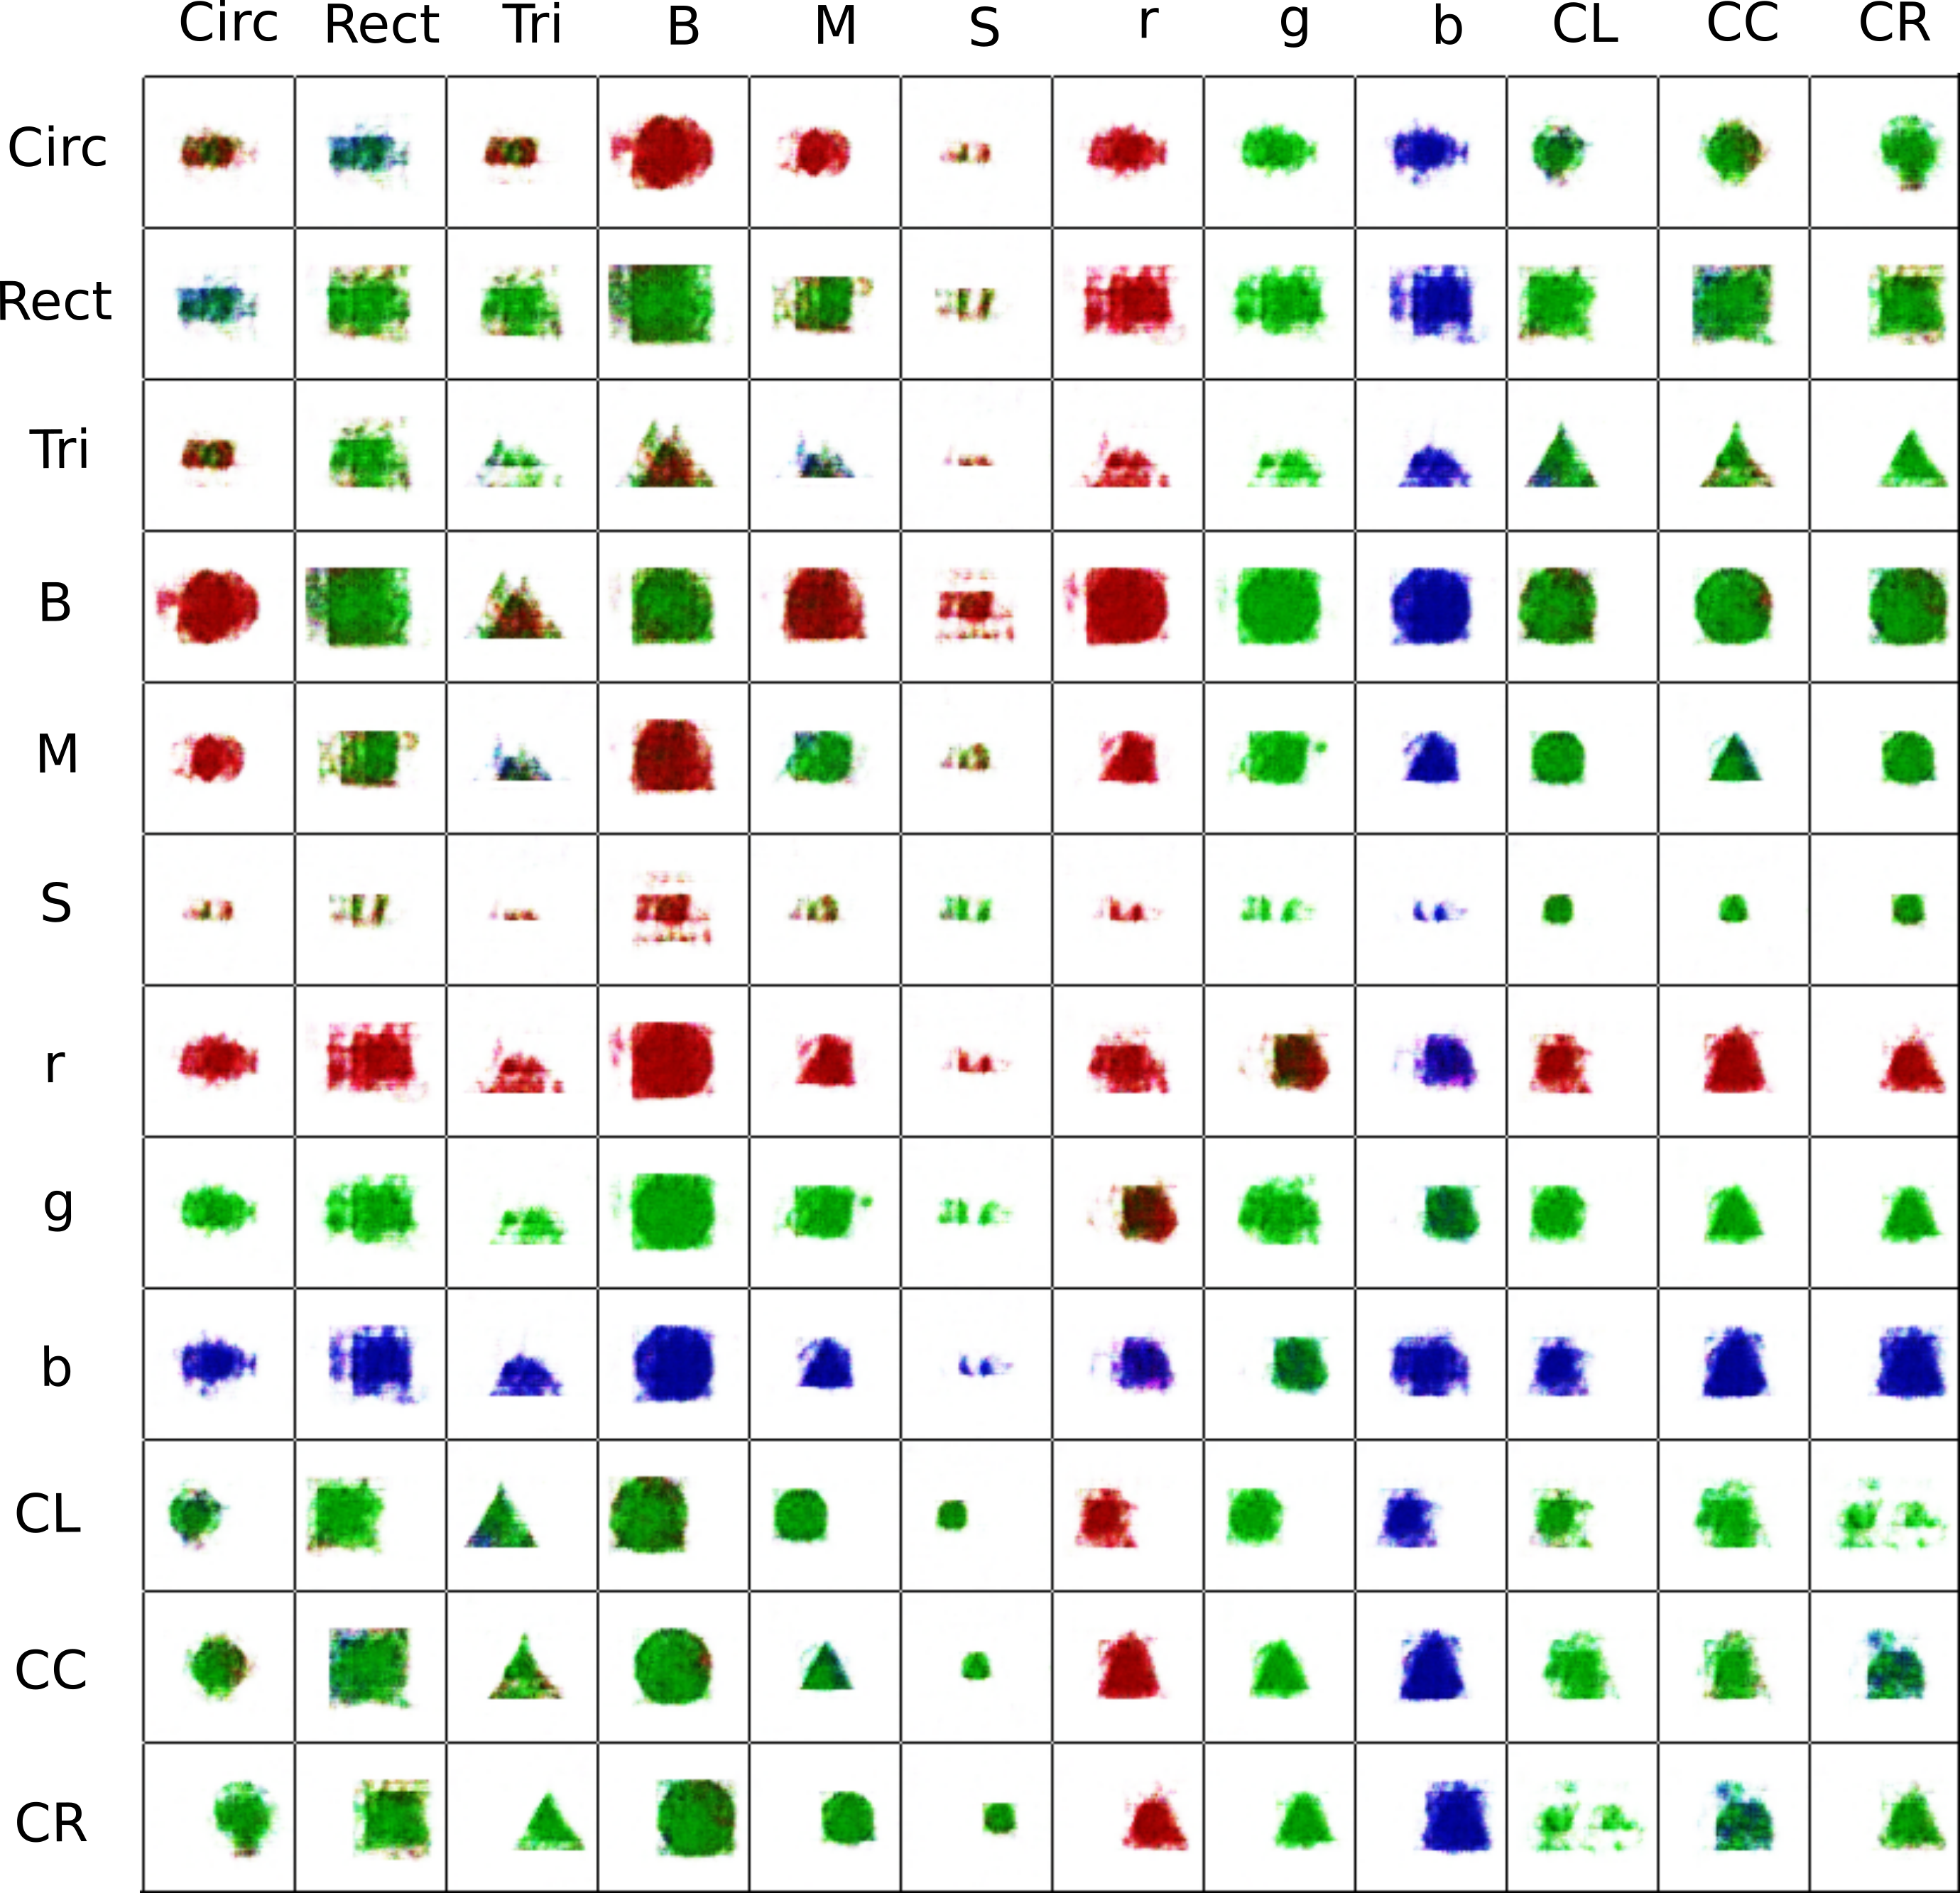
\includegraphics[width=0.75\textwidth]{Figs/shapes/2word333D.png}
\caption{Images generated using word pairs using an embedding size of 296 neurons from experiment 2 run D.}
\label{fig:2word333D}
\end{figure}



\begin{figure}
\centering
\includegraphics[width=\textwidth]{Figs/shapes/2word339A.png}
\caption{Images generated using word pairs using a MAE initialised with random weights for experiment 3 run A.}
\label{fig:2word339A}
\end{figure}

\begin{figure}
\centering
\includegraphics[width=\textwidth]{Figs/shapes/2word339B.png}
\caption{Images generated using word pairs using a MAE initialised with random weights for experiment 3 run B.}
\label{fig:2word339B}
\end{figure}

\begin{figure}
\centering
\includegraphics[width=\textwidth]{Figs/shapes/2word339C.png}
\caption{Images generated using word pairs using a MAE initialised with random weights for experiment 3 run C.}
\label{fig:2word339C}
\end{figure}

\begin{figure}
\centering
\includegraphics[width=\textwidth]{Figs/shapes/2word339D.png}
\caption{Images generated using word pairs using a MAE initialised with random weights for experiment 3 run D.}
\label{fig:2word339D}
\end{figure}

\begin{figure}
\centering
\includegraphics[width=\textwidth]{Figs/shapes/2word339A1.png}
\caption{Images generated using word pairs using a MAE initialised with weights from experiment 1 for experiment 3 run A.}
\label{fig:2word339A1}
\end{figure}

\begin{figure}
\centering
\includegraphics[width=\textwidth]{Figs/shapes/2word339B1.png}
\caption{Images generated using word pairs using a MAE initialised with weights from experiment 1 forexperiment 3 run B.}
\label{fig:2word339B1}
\end{figure}

\begin{figure}
\centering
\includegraphics[width=\textwidth]{Figs/shapes/2word339C1.png}
\caption{Images generated using word pairs using a MAE initialised with weights from experiment 1 for experiment 3 run C.}
\label{fig:2word339C1}
\end{figure}

\begin{figure}
\centering
\includegraphics[width=\textwidth]{Figs/shapes/2word339D1.png}
\caption{Images generated using word pairs using a MAE initialised with weights from experiment 1 for experiment 3 run D.}
\label{fig:2word339D1}
\end{figure}

\begin{figure}
\centering
\includegraphics[width=\textwidth]{Figs/shapes/2word339A2.png}
\caption{Images generated using word pairs using a MAE initialised with weights from experiment 2 for experiment 3 run A.}
\label{fig:2word339A2}
\end{figure}

\begin{figure}
\centering
\includegraphics[width=\textwidth]{Figs/shapes/2word339B2.png}
\caption{Images generated using word pairs using a MAE initialised with weights from experiment 2 forexperiment 3 run B.}
\label{fig:2word339B2}
\end{figure}

\begin{figure}
\centering
\includegraphics[width=\textwidth]{Figs/shapes/2word339C2.png}
\caption{Images generated using word pairs using a MAE initialised with weights from experiment 2 for experiment 3 run C.}
\label{fig:2word339C2}
\end{figure}

\begin{figure}
\centering
\includegraphics[width=\textwidth]{Figs/shapes/2word339D2.png}
\caption{Images generated using word pairs using a MAE initialised with weights from experiment 2 for experiment 3 run D.}
\label{fig:2word339D2}
\end{figure}




\begin{figure}
\centering
\includegraphics[width=\textwidth]{Figs/shapes/2word739A.png}
\caption{Images generated using word pairs using a MAE initialised with random weights for experiment 4 run A.}
\label{fig:2word739A}
\end{figure}

\begin{figure}
\centering
\includegraphics[width=\textwidth]{Figs/shapes/2word739B.png}
\caption{Images generated using word pairs using a MAE initialised with random weights for experiment 4 run B.}
\label{fig:2word739B}
\end{figure}

\begin{figure}
\centering
\includegraphics[width=\textwidth]{Figs/shapes/2word739C.png}
\caption{Images generated using word pairs using a MAE initialised with random weights for experiment 4 run C.}
\label{fig:2word739C}
\end{figure}

\begin{figure}
\centering
\includegraphics[width=\textwidth]{Figs/shapes/2word739D.png}
\caption{Images generated using word pairs using a MAE initialised with random weights for experiment 4 run D.}
\label{fig:2word739D}
\end{figure}


\begin{figure}
\centering
\includegraphics[width=\textwidth]{Figs/shapes/2word739A1.png}
\caption{Images generated using word pairs using a MAE initialised with weights from experiment 1 for experiment 4 run A.}
\label{fig:2word739A1}
\end{figure}

\begin{figure}
\centering
\includegraphics[width=\textwidth]{Figs/shapes/2word739B1.png}
\caption{Images generated using word pairs using a MAE initialised with weights from experiment 1 for experiment 4 run B.}
\label{fig:2word739B1}
\end{figure}

\begin{figure}
\centering
\includegraphics[width=\textwidth]{Figs/shapes/2word739C1.png}
\caption{Images generated using word pairs using a MAE initialised with weights from experiment 1 for experiment 4 run C.}
\label{fig:2word739C1}
\end{figure}

\begin{figure}
\centering
\includegraphics[width=\textwidth]{Figs/shapes/2word739D1.png}
\caption{Images generated using word pairs using a MAE initialised with weights from experiment 1 for experiment 4 run D.}
\label{fig:2word739D1}
\end{figure}

\begin{figure}
\centering
\includegraphics[width=\textwidth]{Figs/shapes/2word739A2.png}
\caption{Images generated using word pairs using a MAE initialised with weights from experiment 2 for experiment 4 run A.}
\label{fig:2word739A2}
\end{figure}

\begin{figure}
\centering
\includegraphics[width=\textwidth]{Figs/shapes/2word739B2.png}
\caption{Images generated using word pairs using a MAE initialised with weights from experiment 2 for experiment 4 run B.}
\label{fig:2word739B2}
\end{figure}

\begin{figure}
\centering
\includegraphics[width=\textwidth]{Figs/shapes/2word739C2.png}
\caption{Images generated using word pairs using a MAE initialised with weights from experiment 2 for experiment 4 run C.}
\label{fig:2word739C2}
\end{figure}

\begin{figure}
\centering
\includegraphics[width=\textwidth]{Figs/shapes/2word739D2.png}
\caption{Images generated using word pairs using a MAE initialised with weights from experiment 2 for experiment 4 run D.}
\label{fig:2word739D2}
\end{figure}


\begin{figure}
\centering
\includegraphics[width=\textwidth]{Figs/shapes/2word739A3.png}
\caption{Images generated using word pairs using a MAE initialised with weights from experiment 3 for experiment 4 run A.}
\label{fig:2word739A3}
\end{figure}

\begin{figure}
\centering
\includegraphics[width=\textwidth]{Figs/shapes/2word739B3.png}
\caption{Images generated using word pairs using a MAE initialised with weights from experiment 3 for experiment 4 run B.}
\label{fig:2word739B3}
\end{figure}

\begin{figure}
\centering
\includegraphics[width=\textwidth]{Figs/shapes/2word739C3.png}
\caption{Images generated using word pairs using a MAE initialised with weights from experiment 3 for experiment 4 run C.}
\label{fig:2word739C3}
\end{figure}

\begin{figure}
\centering
\includegraphics[width=\textwidth]{Figs/shapes/2word739D3.png}
\caption{Images generated using word pairs using a MAE initialised with weights from experiment 3 for experiment 4 run D.}
\label{fig:2word739D3}
\end{figure}


\begin{figure}
\centering
\includegraphics[width=\textwidth]{Figs/shapes/2word739A31.png}
\caption{Images generated using word pairs using a MAE initialised with weights from experiment 1 + 3 for experiment 4 run A.}
\label{fig:2word739A31}
\end{figure}

\begin{figure}
\centering
\includegraphics[width=\textwidth]{Figs/shapes/2word739B31.png}
\caption{Images generated using word pairs using a MAE initialised with weights from experiment 1 + 3 for experiment 4 run B.}
\label{fig:2word739B31}
\end{figure}

\begin{figure}
\centering
\includegraphics[width=\textwidth]{Figs/shapes/2word739C31.png}
\caption{Images generated using word pairs using a MAE initialised with weights from experiment 1 + 3 for experiment 4 run C.}
\label{fig:2word739C31}
\end{figure}

\begin{figure}
\centering
\includegraphics[width=\textwidth]{Figs/shapes/2word739D31.png}
\caption{Images generated using word pairs using a MAE initialised with weights from experiment 1 for experiment 4 run D.}
\label{fig:2word739D31}
\end{figure}





\begin{figure}
\centering
\includegraphics[width=\textwidth]{Figs/shapes/2word739A32.png}
\caption{Images generated using word pairs using a MAE initialised with weights from experiment 2 + 3 for experiment 4 run A.}
\label{fig:2word739A32}
\end{figure}

\begin{figure}
\centering
\includegraphics[width=\textwidth]{Figs/shapes/2word739B32.png}
\caption{Images generated using word pairs using a MAE initialised with weights from experiment 2 + 3 for experiment 4 run B.}
\label{fig:2word739B32}
\end{figure}

\begin{figure}
\centering
\includegraphics[width=\textwidth]{Figs/shapes/2word739C32.png}
\caption{Images generated using word pairs using a MAE initialised with weights from experiment 2 + 3 for experiment 4 run C.}
\label{fig:2word739C32}
\end{figure}

\begin{figure}
\centering
\includegraphics[width=\textwidth]{Figs/shapes/2word739D32.png}
\caption{Images generated using word pairs using a MAE initialised with weights from experiment 2 for experiment 4 run D.}
\label{fig:2word739D32}
\end{figure}



